\documentclass[a4paper,12pt,twoside]{report}
\usepackage{graphicx}
\usepackage{color}
\usepackage{url}
\usepackage{subfigure}
\usepackage[utf8]{inputenc}
\usepackage[T1]{fontenc}
\usepackage{tgpagella}
\usepackage{xstring}
\usepackage{wrapfig}
\usepackage[title,titletoc]{appendix}
%\usepackage{textgreek}
\usepackage{nomencl}
\usepackage{algorithm}
\usepackage{algorithmic}
\usepackage{multicol}
\usepackage{amssymb}
\usepackage{amsthm}
\usepackage{amsmath}
\usepackage{complexity}
%\usepackage{refcheck}
\usepackage[pdfborder=0 0 0,pdftex,unicode]{hyperref}
\DeclareFontShape{OT1}{cmtt}{bx}{n}{<5><6><7><8><9><10><10.95><12><14.4><17.28><20.74><24.88>cmttb10}{}

\newcommand{\myscale}{0.74}
\newcommand{\vect}[1]{\boldsymbol{#1}}
\newcommand{\code}[1]{\texttt{\StrSubstitute{#1}{.}{.\.}}}
\def\.{\discretionary{}{}{}}
\newcommand{\heu}[1]{\texttt{\textit{#1}}}
\newcommand{\dataset}[1]{\texttt{\textit{#1}}}
\newcommand{\jmodule}[1]{\texttt{\textit{#1}}}
\linespread{1.5}
%\onehalfspacing

\renewcommand{\algorithmicrequire}{\textbf{Input:}}
\renewcommand{\algorithmicensure}{\textbf{Output:}}
\renewcommand{\algorithmicforall}{\textbf{for each}}
\renewcommand{\algorithmiccomment}[1]{\textit{// #1}}

\renewcommand{\nomname}{List of Abbreviations}
\makenomenclature

\theoremstyle{definition}
\newtheorem{define}{Definition}[chapter]

% TODO uncomment this to get much shorter ToC
% \setcounter{tocdepth}{1}

\setlength{\hoffset}{-1in} %left margin will be 0, as hoffset is by default 1inch
\setlength{\voffset}{-1in} %analogous voffset
\setlength{\oddsidemargin}{4cm}
\setlength{\evensidemargin}{4cm}
\setlength{\topmargin}{25mm}
\setlength{\footskip}{1cm}
\setlength{\headheight}{0cm}
\setlength{\headsep}{0cm}
\setlength{\marginparwidth}{0cm}
\setlength{\marginparpush}{0cm}
\setlength{\textheight}{23.7cm}
\setlength{\textwidth}{14.5cm}
\let\openright=\clearpage

\def\mfauthor{Matej Vitásek}
\def\mfadvisor{RNDr. Ire\-na Mlýn\-ko\-vá Ph.D.}
\def\mfplacedate{Praha, 2011}

% Tato makra přesvědčují mírně ošklivým trikem LaTeX, aby hlavičky kapitol
% sázel příčetněji a nevynechával nad nimi spoustu místa. Směle ignorujte.
\makeatletter
\def\@makechapterhead#1{
  {\parindent \z@ \raggedright \normalfont
   \Huge\bfseries \thechapter. #1
   \par\nobreak
   \vskip 20\p@
}}
\def\@makeschapterhead#1{
  {\parindent \z@ \raggedright \normalfont
   \Huge\bfseries #1
   \par\nobreak
   \vskip 20\p@
}}
\makeatother

\def\chapwithtoc#1{
  \chapter*{#1}
  \addcontentsline{toc}{chapter}{#1}
}

\begin{document}

\lefthyphenmin=2
\righthyphenmin=2

% -----------------------------------------------------------------------------

%                            FINAL CLEANUP

% - make sure all chapter names are in First Caps
% - make sure all references have a name, like Table 4.3.4 instead of just 4.3.4
% - get rid of all short forms: won't -> will not
% - make sure there are no singletons
% - make sure LaTeX does not complaint much about under/overfullness
% - make sure everything is defined and referenced
% + make sure there is nothing in the bibliography that is unreferenced
% + make sure all the heu/data set names are consistent. This holds especially for GLPK (tool) / Glpk (heu) and FIDAX
% - make sure that when referring to heus in algorithms, e.g. when describing how experimental sets are constructed, we correctly refer to their parameters as described in their pseudocodes
% - the official name for things like OVA1 and 100-100 is (test) data set. Make sure I am not calling it files or anything else.
% - make sure labels have consistent names
% + ratio -> FRACTION of XYZ to fix/remove/...
% + what style of quotation marks to use? (`` and '')

%%% Titulní strana práce ======================================================
\pagestyle{empty}
\begin{center}

\large

Charles University in Prague

\medskip

Faculty of Mathematics and Physics

\vfill

{\bf\Large MASTER THESIS}

\vfill

\centerline{\mbox{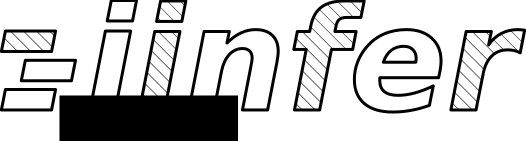
\includegraphics[width=60mm]{logo}}}

\vfill
\vspace{5mm}

{\LARGE \mfauthor}

\vspace{15mm}

% exactly as assigned
{\LARGE\bfseries Inference of XML Integrity Constraints}

\vfill

% Název katedry nebo ústavu, kde byla práce oficiálně zadána
% (dle Organizační struktury MFF UK)
Department of Software Engineering

\vfill

\begin{tabular}{rl}

Supervisor of the master thesis: & 	\mfadvisor \\
\noalign{\vspace{2mm}}
Study programme: & Informatika \\
\noalign{\vspace{2mm}}
Specialization: & ISS \\
\end{tabular}

\vfill

% Zde doplňte rok
\mfplacedate 

\end{center}



\newpage % ============================================================
%%% Následuje vevázaný list -- kopie podepsaného "Zadání diplomové práce".
%%% Toto zadání NENÍ součástí elektronické verze práce, nescanovat.
\openright

\noindent
I would like to thank everyone participating in the jInfer project for creating a~solid foundation for this work, namely Irena Mlýn\-ko\-vá, Mi\-chal Klem\-pa, Má\-rio Mi\-ku\-la, Ro\-bert Sme\-ta\-na and Mi\-chal Švi\-rec. The thanks goes again to Ms. Mlýn\-ko\-vá for supervising this work, as well as everyone reviewing it, in no~particular order Lý\-dia Šva\-ger\-ko\-vá, Mi\-chal Šva\-ger\-ka, Zu\-za\-na Ma\-sá\-ro\-vá, Mi\-chal Ke\-se\-ly and others.

\newpage % ============================================================
%%% Strana s čestným prohlášením k diplomové práci
\vglue 0pt plus 1fill
\noindent
I declare that I carried out this master thesis independently, and only with the cited
sources, literature and other professional sources.

\medskip\noindent
I understand that my work relates to the rights and obligations under the Act No.
121/2000 Coll., the Copyright Act, as amended, in particular the fact that the Charles
University in Prague has the right to conclude a license agreement on the use of this
work as a school work pursuant to Section 60 paragraph 1 of the Copyright Act.

\vspace{10mm}

\hbox{\hbox to 0.5\hsize{%
In ........ date ............
\hss}\hbox to 0.5\hsize{%
signature
\hss}}

\vspace{20mm}



\newpage % ============================================================
%%% Povinná informační strana diplomové práce
\vbox to 0.5\vsize{
\setlength\parindent{0mm}
\setlength\parskip{5mm}

Název práce: Odvozování integritních omezení v XML % TODO how to translate this correctly?

Autor: \mfauthor

Katedra:  Katedra softwarového inženýrství

Vedoucí diplomové práce: \mfadvisor{} % TODO does this have to be here?, Ka\-ted\-ra soft\-wa\-ro\-vé\-ho in\-že\-nýr\-ství

Abstrakt: Tato práce navazuje na dřívější pokusy odvodit (inferovat) schému existujících XML dokumentů. Jelikož je odvozování \textit{struktury} již relativně dobře popsáno, soustředíme se na integritní omezení. Několik jich popisujeme, pozornost pak soustředíme na ID/\.IDREF/\.IDREFS atributy z DTD. Na bázi článku od Barbosa a Menelzon stavíme heuristický přístup k problému hledání optimální sady ID atributů, jeho funkčnost a vhodnost pak ověřujeme na škále experimentů.

Klíčová slova:  XML, ID atributy, odvozování

\vss}\nobreak\vbox to 0.49\vsize{
\setlength\parindent{0mm}
\setlength\parskip{5mm}

Title:  Inference of XML Integrity Constraints

Author: \mfauthor

Department: Department of Software Engineering

Supervisor: \mfadvisor{} % TODO does this have to be here?, Department of Software Engineering

Abstract: In this work we expand upon the previous efforts to extract (infer) schema information from existing XML documents. We find the inference of \textit{structure} to be sufficiently researched and focus further on integrity constraints. After briefly introducing some of them we turn our attention to ID/\.IDREF/\.IDREFS attributes in DTD. Building on the research by Barbosa and Menelzon we introduce a heuristic approach to the problem of finding optimal ID set. The approach is evaluated and tuned in a wide range of experiments.

Keywords: XML, ID attributes, inference

\vss}

\newpage

%%% Strana s automaticky generovaným obsahem diplomové práce. U matematických
%%% prací je přípustné, aby seznam tabulek a zkratek, existují-li, byl umístěn
%%% na začátku práce, místo na jejím konci.

\openright
\pagestyle{plain}
\setcounter{page}{1}
\tableofcontents

% =============== TEXT ================
\newpage

\chapwithtoc{Preface}
\label{chapter-preface}

Along with technologies such as SQL/noSQL databases, proprietary binary file formats, plain-text configuration files and JSON, XML is one of the leading formats for storing structured data. However, even though languages such as DTD and XML Schema to describe XML structure exist for a long time, most of the documents use outdated or no schema at all (\cite{1802522}). To tackle this problem one may employ reverse-engineering techniques to infer the schema from existing documents, such as those described in \cite{ahonen, bex, vyhnanovska}. In particular, \cite{archdoc} introduces the jInfer schema inference framework, dealing primarily with the structural parts of the schema: how all the elements, attributes and text data are to be organized in an XML document conforming to that schema. Inference of this kind of structural information was greatly improved in \cite{anti}.\\

But the schema is not the only constraint that can be imposed on an XML document. Any textual or numerical value featured in the document may be subject to type constraints, such as the requirement to conform to a specific regular expression. Furthermore, the concept of \textit{keys} and \textit{foreign keys}, well known from the relational database world, applies to schemas as well and will be the topic of this work. One could go even further and try to find even more sophisticated relations in the data, such as \textit{functional dependencies} well researched in \cite{sviro}.\\

From all the constraints that can be applied to an XML document by means of its schema, this work will focus on keys and foreign keys. Most important concepts in this field are introduced in \cite{keX} and formalized in the notions of \texttt{ID/IDREF/IDREFS} attributes in DTD and XSD and \texttt{xs:key/xs:keyref} structures in XSD (both in \cite{Bray:08:EML}).\\

The scope of this work is finally limited to the inference of \texttt{ID/IDREF/IDREFS} from existing XML documents. ID attributes were chosen over \texttt{xs:key} because the preliminary research found that while it is possible to find real-life XML data with schemas containing \texttt{xs:key} structure, schemas with ID attributes are much more common and it is much easier to obtain large data sets for experiments. % TODO something like even the search for ID sets is interesting enough?

\section{Structure of the thesis}

The thesis will be structured as follows.

First, we will introduce a few notions required throughout the work, such as XML tree, ID attributes, ID sets, linear programming and mixed integer problem. 

We will then review approaches to ID attribute search from previous articles on this topic and formulate the problem of finding the optimal ID set.

This will lead us to the NP-complete problem of Maximum Independent Set, where we will inspect the approaches to solving it.

We will discuss a closely related Mixed Integer Problem and show that by solving MIP we can solve the Maximum Independent Set and thus the original problem of optimal ID set.

Afterwards, we will show how to use an external MIP solver, demonstrate that this can take too long and how to use a heuristic approach to find good solutions much faster.

An extension to jInfer for finding ID attributes using MIP solver and a combination of heuristics will be presented and experimentally evaluated in the closing chapters.

\section{Conventions}

As usual, source code excerpts, class, field and method names shall be written in fixed-width font, such as \texttt{get\-Heu\-ris\-tic()}. Names of specific heuristics will be written like \heu{Mutation}. Name of test data sets will be written like \dataset{OVA1}.\\

Pseudocode examples such as the one in Listing \ref{listing-example} will always be presented in a functional way, with inputs and outputs of the function clearly marked in the beginning.

\begin{algorithm}
\caption{Example Algorithm}
\label{listing-example}
\begin{algorithmic}
\REQUIRE $I$ input data
\REQUIRE $n$ maximum number of iterations
\ENSURE results found
\FOR{$i = 1 \to n$}
  \STATE \COMMENT{try to find a solution}
  \STATE $attempt \gets $ calculate possible solution from $I$
  \IF{$attempt$ is a valid solution}
    \RETURN $attempt$
  \ENDIF
  \RETURN ``solution not found''
\ENDFOR
\end{algorithmic}
\end{algorithm}

There is a list of abbreviations following the bibliography in Listing \ref{chapter-list-abbreviations}.\\

Please note that throughout this work we will be explicitly ignoring the $\mathcal{O}()$ complexities of algorithms we use. This is because the algorithms we use are by principle strongly stochastic and their performance often depends on behavior of external tools, which we regarded as black boxes and mostly ignored their inner workings.

\chapter{Definitions}

TODO we shall introduce a number of definitions, some only auxiliary, some necessary in the whole work

\section{XML Tree}

TODO from FIDAX or wherever

\subsection{Element, Attribute}

TODO

\section{ID, IDREF, IDREFS Attributes}

TODO according to specification

\section{XML Keys}

TODO

\subsection{According to Specification}

TODO compare them to ID attributes

\subsection{According to \cite{keX}}

TODO show how a XML key is defined using the keX notation % this is a terrible sentence

\section{Attribute Mappings}

TODO \nomenclature{AM}{Attribute Mapping}

\subsection{Attribute Mapping Model}

TODO

\section{ID Set}

TODO

\section{Attribute Mapping Weight}

TODO

\subsection{Support}

TODO

\subsection{Coverage}

TODO

\chapter{Research}

According to the article \cite{fidax}, ...

TODO talk about FIDAX
To the best of our knowledge, there are no other articles dealing with this problem.

TODO talk about Fajt - but that's different, that's keys
TODO add citation for Fajt

\section{Independent Set}

TODO define IS + MIS rigorously

TODO other approaches to max IS


\chapter{MIP Approach}
\label{chapter-mip}

In this chapter we introduce a new approach to finding maximum ID sets. First, we transform the problem formulation to maximum weighted IS problem formulation. Then we transform this into a MIP formulation, and demonstrate how this can be solved using a solver such as GLPK. \nomenclature{GLPK}{GNU Linear Programming Kit}
We will continue by applying heuristical approaches to improve the performance of the process.

\section{ID Set to IS Formulation}

Given $C = \{m_1, \ldots, m_n\}$ a set of all AMs in a document, we construct a graph $G = (V,E)$ as follows. For each AM $m_i \in C$ we create a vertex $v_{name(m_i)}$. Two vertices $v_{name(m_i)}$ and $v_{name(m_j)}$ shall be connected by an edge iff they cannot share the same ID set, either because they have the same type ($\tau(m_i) = \tau(m_j)$), or their images intersect ($\iota(m_i) \cap \iota(m_j) \neq \emptyset$). Weight of a vertex $v_{name(m_i)}$ is the weight of the attribute mapping: $w(v_{name(m_i)}) = weight(m_i)$.

Now finding the maximum weighted IS in $G$ finds the maximum (optimal) ID set in the original document.

\section{IS to MIP Formulation}

Given a graph $G = (V,E)$ with a weight function $w: V \rightarrow \mathbb{R}$, we introduce a binary variable $x_i$ for each vertex $v_i \in V$ and an inequality constraint $x_i + x_j \leq 1$ for each edge $e = (v_i, v_j) \in E$. Furthermore we introduce an objective function in form $\sum_{x_i} x_i w(v_i)$.

It is obvious that the objective function and all the constraints consitute a MIP instance, and that solving it finds the maximum weigthed IS in $G$.

\section{Finding ID Sets With GLPK}
\label{section-mip-glpk}

By chaining these two translations we can create a MIP formulation for a given set of AMs from a document. Solving this MIP instance will give us the optimal ID set for this document.

GLPK \cite{glpk} is a multi-platform, multi-purpose solver well suited for this task. It uses the Simplex method to solve LP problems and \textit{Branch \& Bound} (see \cite{land60a} for details) for MIP. An advantage of using \textit{Branch \& Bound} is that while traversing the \textit{search tree} it finds intermittent, sub-optimal solutions. It is thus possible to limit the total search time and instead of the optimum take the best solution found so far.\\

We will now demonstrate the full process of finding the optimal ID set of an example XML file using GLPK.

\subsection{Example}

Consider again our XML file fragment.

\begin{verbatim}
<x>
  <y a="1" b="2"/>
  <y a="3" c="4"/>
  <y/>
  <z a="1"/>
</x>
\end{verbatim}

Recall that attribute mappings in this example are $C = \{M_{y}^{a}, M_{y}^{b}, M_{y}^{c}, M_{z}^{a}\}$. Corresponding vertices in the IS formulation will be $V = \{v_{y-a}, v_{y-b}, v_{y-c}, v_{z-a}\}$. Edges in the IS formulation will be the following.

\begin{eqnarray*}
(v_{y-a},v_{y-b}) \\
(v_{y-a},v_{y-c}) \\
(v_{y-b},v_{y-c}) \\
(v_{y-a},v_{z-a}) \\
\end{eqnarray*}

First three edges are due to the type collision ($y$), the last one is due to $\iota(M_{y}^{a}) \cap \iota(M_{z}^{a}) = \{1\}$. The graph $G$ constructed in this way is in Figure \ref{image-mip-is-graph}.

\begin{figure}
  \caption{IS Representation Graph}
  \label{image-mip-is-graph}
  \centering
	\includegraphics[width=.25\textwidth]{images/is-representation}
\end{figure}

The next step is the MIP formulation. We do not need to translate from the IS formulation, as the translation from ID set formulation is straightforward, too. For each AM $m$ there will be one binary variable $x_{name(m)}$. Objective function coefficients in vector $\mathbf{c}$ will be weights of respective mappings. For each pair of AMs $m_1, m_2$ that cannot share the same ID set there shall be a row in matrix $A$ representing the inequality $x_{name(m_1)} + x_{name(m_2)} \leqslant 1$. $\mathbf{b}$ will be a vector of ones with corresponding length.

\[
\mathbf{x} =
\begin{bmatrix}
x_{y-a} \\
x_{y-b} \\
x_{y-c} \\
x_{z-a} \\
\end{bmatrix},
\mathbf{c} = 
\begin{bmatrix}
weight(M_{y}^{a}) \\
weight(M_{y}^{b}) \\
weight(M_{y}^{c}) \\
weight(M_{z}^{a}) \\
\end{bmatrix} =
\begin{bmatrix}
0.2 \\
0.2 \\
0.6 \\
0.4 \\
\end{bmatrix},
\mathbf{b} =
\begin{bmatrix}
1 \\
1 \\
1 \\
1 \\
\end{bmatrix},
A =
\begin{pmatrix}
0 & 1 & 1 & 0 \\
1 & 0 & 1 & 0 \\
1 & 1 & 0 & 0 \\
1 & 0 & 0 & 1 \\
\end{pmatrix}
\]

The problem now is, recall, to solve the following.

\begin{eqnarray*}
\max_{x} z & = & \mathbf{c}^{\mathrm{T}}\mathbf{x} \\
s.t.\, A\mathbf{x} & \leqslant & \mathbf{b} \\
\end{eqnarray*}

In GLPK \textit{MathProg} language (see \cite{mathprog}), this translates to the following formulation.

\begin{scriptsize}
\begin{verbatim}
set AMs;
param Weight {i in AMs};
var x {i in AMs} binary;
maximize z: sum {i in AMs} x[i] * Weight[i];
s.t. c1: x['y-a'] + x['y-b'] <= 1;
s.t. c2: x['y-a'] + x['y-c'] <= 1;
s.t. c3: x['y-b'] + x['y-c'] <= 1;
s.t. c4: x['y-a'] + x['z-a'] <= 1;
data;
set AMs := y-a y-b y-c z-a;
param Weight :=
y-a 0.6
y-b 0.2
y-c 0.2
z-a 0.4;
end;
\end{verbatim}
\end{scriptsize}

We can use this as an input for the GLPK solver, and we get the solution.

\begin{scriptsize}
\begin{verbatim}
...
Problem:    glpk_input
Rows:       5
Columns:    4 (4 integer, 4 binary)
Non-zeros:  12
Status:     INTEGER OPTIMAL
Objective:  z = 0.6 (MAXimum)

...

   No. Column name       Activity     Lower bound   Upper bound
------ ------------    ------------- ------------- -------------
     1 x[y-a]       *              1             0             1 
     2 x[y-b]       *              0             0             1 
     3 x[y-c]       *              0             0             1 
     4 x[z-a]       *              0             0             1 

...
\end{verbatim}
\end{scriptsize}

This output tells us that the solution is $x_{y-a} = 1$, $x_{y-b} = 0$, $x_{y-c} = 0$ and $x_{z-a} = 0$. This means that the optimal ID set with maximum weight contains only the $M_{y}^{a}$ attribute mapping.\\

It is obvious that this approach works and for any possible input we can let GLPK find the optimal solution. However, sometimes it takes too long to find the optimum (see e.g. Section \ref{section-glpk-comparison}), we should try to improve this process.

\section{Heuristics}
\label{section-mip-heuristics}

The definition of \textit{heuristic} or \textit{heuristic algorithm} varies from one source to another. We shall be using it roughly in the following sense.

\begin{define}[Heuristic]
	Is an approach to problem solving based on prior experience, educated guess or common knowledge.
\end{define}

\begin{define}[Heuristic Algorithm]
	Is an algorithm that, in a reasonably short time, will generate a good, maybe even optimal solution to an optimization problem. However, it won’t provide any formal guarantee about its quality.
\end{define} 

This definion of heuristic algorithm coming from \cite{heu-lecture} is rather vague, however, it will be sufficient for us.

An example of a heuristic is the commonly used approach of \textit{trial and error}: after a failed attempt, change something and try again. We will see many more heuristics later in this chapter.

While a heuristic algorithm can be seen as a tool designed to solve one specific problem, the notion of a \textit{metaheuristic} reminds of a recipy to solve a whole family of problems. We shall be using the metaheuristic presented in Figure \ref{image-metaheuristic} to find optimal ID sets in this work. But before we start describing its structure and components, we need to introduce some more notions.

\begin{figure}
  \caption{Metaheuristic schema}
  \label{image-metaheuristic}
  \centering
    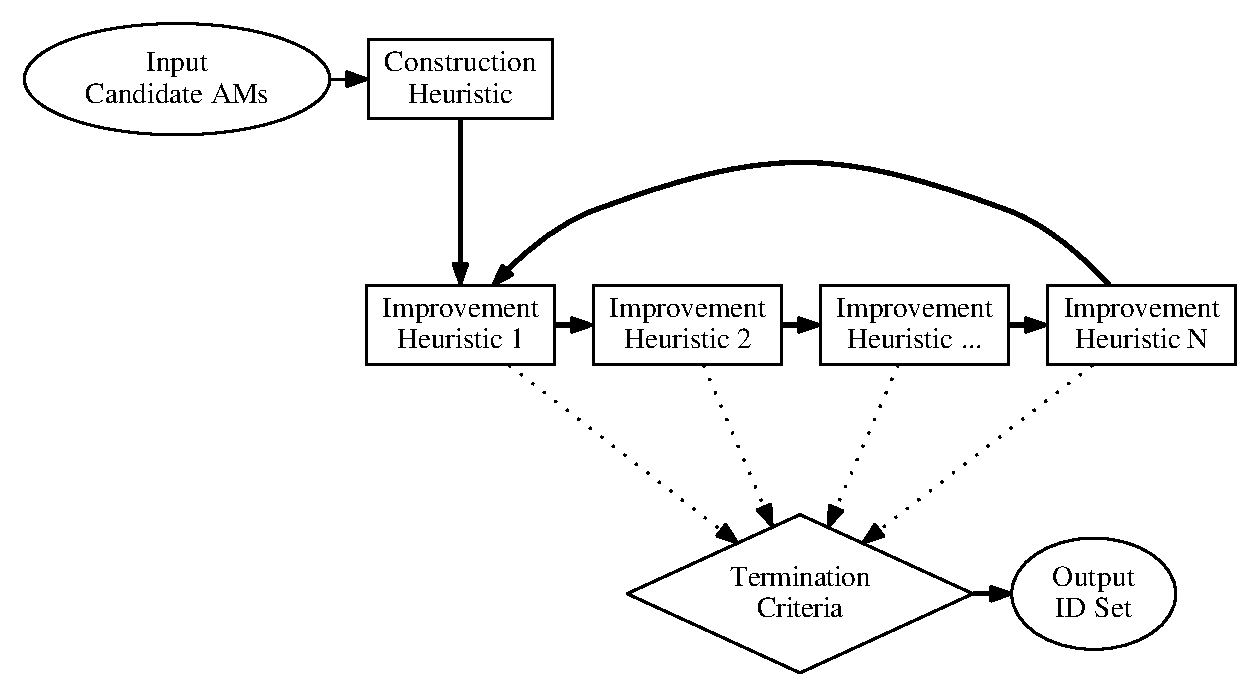
\includegraphics[width=\textwidth]{images/metaheuristic}
\end{figure}

\begin{define}[Solution Space, Solution Quality]
	Solution space in general is the set of all permissible solutions (not violating any constraints). In the specific case of a MIP formulation it is the set of all $\mathbf{x}$ subject to $A\mathbf{x} \leqslant \mathbf{b}$. Every solution in the solution space has its \textit{quality}, in case of MIP for solution $\mathbf{x}$ it is the value of the objective function in $\mathbf{x}$.
\end{define}

\begin{define}[Solution Neighborhood]
	Neighborhood of a solution $\mathbf{x}$ in the solution space are all the other solutions close to $\mathbf{x}$ according to some metric.
\end{define}

The precise definition of the neighborhood is always adjusted according to specific needs. However, the neighborhood should be defined so that is \textit{continuous} (with respect to quality) to be useful. The exact reasons for this requirement are sketched in Section \ref{section-mip-ihs}.

\begin{define}[Solution Pool, Incumbent Solution]
	\textit{Solution pool} (sometimes called pool of feasible solutions or feasible pool) is simply a set of solutions of different qualities that were found in one of the stages of the metaheuristic. The solution(s) with the highest quality is (are) called the \textit{incumbent} solution(s).
\end{define}

A quick reminder of what we are trying to solve using our metaheuristic: given a list of AMs with weights, find a non-conflicting subset maximizing the sum of weights in the subset. We will now describe its structure, please refer again to Figure \ref{image-metaheuristic}.

First we take the list of candidate AMs and ask a \textit{construction heuristic} (see Section \ref{section-mip-chs}) to provide us with a pool of solutions. Then, in a loop, we use this pool as input for \textit{improvement heuristics} (see Section \ref{section-mip-ihs}) and in turns ask them to improve it. All the time we check whether some \textit{termination criteria} are met, and if it is so, we terminate the metaheuristic. The incumbent solution from the last pool is then declared the Output ID set.\\

The notion of metaheuristic covers a wide range of topics in the field of heuristics, such as Tabu Search (see \cite{Glover:1997:TS:549765}), Ant Colony Optimization (see \cite{dorigo2004ant}) or Genetic Algorithms (see e.g. \cite{goldberg1989genetic}), to name a few.\\

We will now introduce the heurisitics we have implemented to use in our metaheuristic for finding optimal ID sets.

\subsection{Constructions Heuristics}
\label{section-mip-chs}
\nomenclature{CH}{Construction Heuristic}

When we start to solve a problem using a metaheuristic approach, at first we have no solutions at all. The purpose of a construction heuristic (CH) is then to provide us with at least some solution. This may or may not be already the optimum, in the latter case it will be improved on later using improvement heuristics (IH). Some IHs can profit from a pool of several sub-optimal solutions, and some CHs can produce this pool from them.

\subsubsection{\heu{FIDAX}}
\label{section-mip-fidax}

The first construction heuristic is the algorithm described in \cite{fidax} (we shall call it \heu{FIDAX} from now on). It can trivially be used to give us one feasible solution - it is, after all, a deterministic heuristic algorithm.

The pseudocode of this CH (taken from the original article with trivial modifications without changing the logic) is in Listing \ref{listing-ch-fidax}.

\begin{algorithm}
\caption{\heu{FIDAX} CH}
\label{listing-ch-fidax}
\begin{algorithmic}
\REQUIRE $C$ list of candidate AMs
\ENSURE a feasible solution
\STATE $C' \gets C$ sorted by decreasing size
\STATE Compute the weight $w(m)$ of each $m$ in $C$
\FORALL{$t$ in $\Sigma^E$}
  \STATE Let $m$ be a \textbf{highest-weight} mapping of type $t$ in $C'$
  \STATE Remove from $C'$ all mappings of type $t$ except $m$
\ENDFOR
\FORALL{$m$ in $C'$}
  \STATE $S \gets$ all mappings in $C$ whose images intersect $\iota(m)$
  \IF{$w(m) > \sum_{p \in S} w(p)$}
    \STATE remove all $p \in S$ from $C'$
  \ELSE
    \STATE remove $m$ from $C'$
  \ENDIF
\ENDFOR
\RETURN $C'$
\end{algorithmic}
\end{algorithm}

\subsubsection{\heu{Random}}
\label{heu-ch-random}

One of the most natural heuristics when dealing with the ID set problem can be described as follows: select from candidate AMs at random, if possible (addition would not violate the ID set condition) add them to the solution. This is obviously a hungry heuristic.

The advantages of this trivial heuristic are simplicity, speed and ease with which it can create a pool of variable solutions, almost for free. As we will see later in the experiments (Section \ref{section-experiments-random-fuzzy-fidax}), it performs surprisingly well.

See the Listing \ref{listing-ch-random} for its pseudocode.

\begin{algorithm}
\caption{\heu{Random} CH}
\label{listing-ch-random}
\begin{algorithmic}
\REQUIRE $N$ required size of pool
\REQUIRE $C$ list of candidate AMs
\ENSURE pool of $N$ feasible solutions
\STATE $r \gets $ empty pool
\FOR{$i = 1 \to N$}
  \STATE \COMMENT{create 1 solution}
  \STATE $s \gets $ empty solution
  \WHILE{$s$ is a feasible ID set}
    \STATE $a \gets $ pick at random from $C \backslash S$
    \STATE $s \gets s \cup a$
  \ENDWHILE
  \STATE $r \gets r \cup s$
\ENDFOR
\RETURN $r$
\end{algorithmic}
\end{algorithm}

\subsubsection{\heu{Fuzzy}}
\label{heu-ch-fuzzy}

\heu{Fuzzy} is an improvement over the \heu{Random} CH: the next AM to be added is selected based on \textit{weighted} instead of uniform random. The weight used here is the usual weight of an AM as defined in Section \ref{section-definitions-weight}. Because of the randomness involved in the choice, we can again easily create a pool of solutions this way.

This is again a hungry heuristic, the Listing \ref{listing-ch-fuzzy} contains its pseudocode.

\begin{algorithm}
\caption{\heu{Fuzzy} CH}
\label{listing-ch-fuzzy}
\begin{algorithmic}
\REQUIRE $N$ required size of pool
\REQUIRE $C$ list of candidate AMs
\ENSURE pool of $N$ feasible solutions
\STATE $r \gets $ empty pool
\FOR{$i = 1 \to N$}
  \STATE \COMMENT{create 1 solution}
  \STATE $s \gets $ empty solution
  \STATE $C' \gets C$

  \WHILE{$C' $ not empty}
    \STATE $a \gets $ pick at weighted random from $C'$
    \IF{$s \cup a$ is a feasible ID set}
      \STATE $s \gets s \cup a$
      \STATE $C' \gets C' \backslash a$
    \ENDIF
    \FORALL{$c \in C'$}
      \IF{$s \cup c $ is \textbf{not} a feasible ID set}
        \STATE \COMMENT {if $c$ cannot be possibly added anymore}
        \STATE $C' \gets C' \backslash c$
      \ENDIF
    \ENDFOR
  \ENDWHILE

  \STATE $r \gets r + s$
\ENDFOR
\RETURN $r$
\end{algorithmic}
\end{algorithm}

\subsubsection{\heu{Incremental}}

This trivial heuristics sorts all candidate AMs by their decreasing weights (Section \ref{section-definitions-weight}) and then tries to iteratively add them to solution, if possible. This way it can create only one solution, and again, this is a hungry heuristic.

See Listing \ref{listing-ch-incremental} for its pseudocode.

\begin{algorithm}
\caption{\heu{Incremental} CH}
\label{listing-ch-incremental}
\begin{algorithmic}
\REQUIRE $C$ list of candidate AMs
\ENSURE a feasible solution
\STATE $C' \gets $ sort $C$ by decreasing weight
\STATE $s \gets $ empty solution
\FORALL{$c \in C'$}
  \IF{$s \cup c$ is a feasible ID set}
    \STATE $s \gets s + c$
  \ENDIF
\ENDFOR
\RETURN $s$
\end{algorithmic}
\end{algorithm}

\subsubsection{\heu{Removal}}

This is basically a reversal of the idea from the \heu{Incremental} heuristic - start with a solution containing all the candidate AMs. This probably does not satisfy the ID set condition. Therefore, sort them by increasing size and start removing them from the solution, until it satisfies the ID set condition. Again, this is a hungry heuristic returning only one solution.

See Listing \ref{listing-ch-removal} for its pseudocode.

\begin{algorithm}
\caption{\heu{Removal} CH}
\label{listing-ch-removal}
\begin{algorithmic}
\REQUIRE $C$ list of candidate AMs
\ENSURE a feasible solution
\STATE $C' \gets $ sort $C$ by increasing weight
\STATE $s \gets C'$
\FORALL{$c \in s$}
  \IF{$s$ is a feasible ID set}
    \RETURN $s$
  \ENDIF
  \STATE $s \gets s \backslash c$
\ENDFOR
\end{algorithmic}
\end{algorithm}

\subsubsection{Truncated Branch \& Bound - \heu{Glpk}}

This construction heuristic will be called \heu{Glpk} from now on, for it is basically a time-constrained run of GLPK. Recall that GLPK uses a the \textit{Branch \& Bound} algorithm that produces feasible solutions even before the optimum is found. Limiting the run time gives us the best solution found so far, which means this is a construction heuristic.

To be able to create a pool of solutions, the GLPK input in MathProg langauge is always randomly shuffled by changing the order in which variables and constraints appear. This is causes the solver to explore the search tree in various orders, producing different solution in each of the time-constrained runs.

\subsection{Improvement Heuristics}
\label{section-mip-ihs}

\nomenclature{IH}{Improvement Heuristic}

Improvement heuristics in general start with a solution pool, attempt to improve one or more solutions in it and then return this improved pool in the end. We will need two notions to describe their behavior.

\paragraph{Intensification}

is the attempt to move the solution towards the nearby local optimum in the solution space.

\paragraph{Diversification}

is the attempt to move the solution away (escape) from from the local optimum, to be able to explore more of the solution space when the metaheuristic starts stagnating.\\

A metaheuristic needs to combine intensification and diversification tendencies to explore the solution space and at the same time arrive at a local optimum. Recall the requirement for the solution space to be continuous in terms of quality: this guarantees that as we approach a solution $\mathbf{x}$, the quality of solutions we encounter approaches the quality of $\mathbf{x}$.

\subsubsection{\heu{Identity}}

This ultimately trivial improvement heuristics does nothing. It simply returns the feasible pool unchanged. For the sake of completeness, see its Listing \ref{listing-ih-identity}.

\begin{algorithm}
\caption{\heu{Identity} IH}
\label{listing-ih-identity}
\begin{algorithmic}
\REQUIRE $FP$ pool of feasible solutions
\ENSURE the same pool of feasible solutions
\RETURN $FP$
\end{algorithmic}
\end{algorithm}

\subsubsection{\heu{Remove Worst}}

This trivial IH tries to improve the solution pool by removing the worst solution (i.e. the one with the lowest quality). This is interesting in cooperation with other improvement heuristics that increase the solution pool size, to keep it from growing by pruning inferior solutions.

See Listing \ref{listing-ih-removeworst} for details.

\begin{algorithm}
\caption{\heu{Remove Worst} IH}
\label{listing-ih-removeworst}
\begin{algorithmic}
\REQUIRE $FP$ pool of feasible solutions
\ENSURE pool of feasible solutions
\STATE $s_{min} \gets $ solution with the lowest weight $\in FP$
\RETURN $FP \backslash s_{min}$
\end{algorithmic}
\end{algorithm}

\subsubsection{\heu{Random Remove}}

This is again a rather trivial diversification improvement heuristic. By removing a random subset of specified size from each solution in the pool, it provides the variability needed to escape from local optima in the solution space.

The number of AMs to remove from each solution is specified as fraction from $(0, 1)$ of the solution size (number of AMs in solution). For example, \heu{Random Remove} with $fraction = 0.1$ would remove 1 random AM from a solution containing 10 AMs and 2 from a solution containing 17 AMs (due to rounding).

This heuristic returns a pool of solutions of the same size as it got on its input.

See Listing \ref{listing-ih-randomremove} for pseudocode.

\begin{algorithm}
\caption{\heu{Random Remove} IH}
\label{listing-ih-randomremove}
\begin{algorithmic}
\REQUIRE $FP$ pool of feasible solutions
\REQUIRE $k \in (0,1)$ fraction of AMs to remove from each $s \in FP$
\ENSURE pool of feasible solutions
\FORALL{$s \in FP$}
  \STATE $K \gets k * |s|$
  \STATE remove $K$ random AMs from $s$
\ENDFOR
\RETURN $FP$
\end{algorithmic}
\end{algorithm}

\subsubsection{\heu{Hungry}}

This simple improvement heuristic assumes that the solutions in the pool are not ``complete'', i.e. there are AMs that could be added to them without violating the ID set condition.

\heu{Hungry} tries to improve each solution in the feasible pool in the following way. It orders all candidate AMs not present in the solution by decreasing weight. Afterwards, it iteratively tries to extend the solution with these AMs, taking care not to violate the ID set condition. The resulting solution (whether any AMs were added or not) is then returned to the pool. This is then intensification, and Listing \ref{listing-ih-hungry} captures the process.\\

\begin{algorithm}
\caption{\heu{Hungry} IH}
\label{listing-ih-hungry}
\begin{algorithmic}
\REQUIRE $FP$ pool of feasible solutions
\REQUIRE $C$ list of candidate AMs
\ENSURE pool of feasible solutions
\FORALL{$s \in FP$}
  \STATE \COMMENT {improve a single solution}
  \STATE $C' \gets C \backslash s$
  \STATE $C' \gets C'$ sorted by decreasing weight
  \FORALL{$c \in C'$}
    \IF{$s \cup c$ is a feasible ID set}
      \STATE $s \gets s \cup c$
    \ENDIF
  \ENDFOR
\ENDFOR
\RETURN $FP$
\end{algorithmic}
\end{algorithm}

The following three IHs: \heu{Mutation}, \heu{Crossover} and \heu{Local Branching} are inspired by \cite{heu-lecture}.

\subsubsection{\heu{Mutation}}

\heu{Mutation} is based on the following idea. We assume that an incumbent solution may already contain some AMs belonging to the optimal solution. We will take a random guess and fix some of these AMs: add new constraints to the MIP formulation fixing values of the respective variables to 1.

This new formulation contains less free variables and should be easier to solve, probably even to optimum. We run GLPK again using this constrained formulation, enforcing again a time limit. Solution found this way is a feasible solution of the original problem, however the optimum is not necessarily the same as in unconstrained formulation. It is an intensification approach: we limit the search to the neighborhood of an already found solution.\\

\heu{Mutation} changes the MIP formulation in following way. For every AM $AM_F$ fixed to appear in the solution a following constraint is added to GLPK input:
\[s.t. f_{index}: x['name(AM_F)'] = 1;\]
$index$ is a unique integer to number all the constraints.

Additionaly, every other mapping $AM_i$ colliding with $AM_F$ ($\iff \iota(AM_F) \cap \iota(AM_i) \neq \emptyset$) will cause the following constraint to be added:
\[s.t. f_{index}: x['name(AM_i)'] = 0;\]
And the original constraint in form:
\[s.t. c_{index}: x['name(AM_F)'] + x['name(AM_i)'] <= 1;\]
will not be included.\\

Listing \ref{listing-ih-mutation} captures the process of randomly selecting a specified fraction of AMs of the incumbent solution to fix, then running GLPK again. \heu{Mutation} requires pool of at least one solution as input, and adds the improved solution to the result pool.

\begin{algorithm}
\caption{\heu{Mutation} IH}
\label{listing-ih-mutation}
\begin{algorithmic}
\REQUIRE $FP$ pool of feasible solutions
\REQUIRE $k$ fraction of AMs to fix
\ENSURE pool of feasible solutions
\STATE $incumbent \gets $ incumbent solution in $FP$
\STATE $K \gets k * |incumbent|$
\STATE fix $K$ random AMs from $incumbent$ in GLPK problem formulation
\STATE $improved \gets $ run GLPK
\RETURN $FP \cup improved$
\end{algorithmic}
\end{algorithm}

\subsubsection{\heu{Crossover}}

This improvement heuristic expands on the idea of \heu{Mutation}. But, instead of randomly selecting AMs in the incumbent solution, it looks for commonalities among the solutions in the pool. This is based on the hope that if more solutions agree on the same AMs, those are probably included in the optimal solution too.

\heu{Crossover} takes a parameter - fraction of solutions in the pool among which to look for commonalities. AMs found in every one of them are fixed in the modified MIP formulation the same way as in \heu{Mutation}. This again amounts to an intensification tendency.

Listing \ref{listing-ih-crossover} captures the process. \heu{Crossover} requires at least one solution in the pool, but to work properly, more are needed. Solutions are picked at random from the pool, common AMs found and fixed. GLPK is run again (with a time constraint) and the improved solution is added to the result pool.

\begin{algorithm}
\caption{\heu{Crossover} IH}
\label{listing-ih-crossover}
\begin{algorithmic}
\REQUIRE $FP$ pool of feasible solutions
\REQUIRE $k$ fraction of solutions among which to look for commonalities
\ENSURE pool of feasible solutions
\STATE $K \gets k * |FP|$
\STATE $FP' \gets K$ random solutions $\in FP$
\STATE $am \gets$ AMs found in all solutions $\in FP'$
\STATE fix $am$ in GLPK problem formulation
\STATE $improved \gets $ run GLPK
\RETURN $FP \cup improved$
\end{algorithmic}
\end{algorithm}

\subsubsection{\heu{Local Branching}}

\heu{Local Branching} is another intensification heuristic. This time the neighborhood being searched is defined by edit distance.

The incumbent solution is represented by a vector $\mathbf{x}_{INCUMBENT}$ of ones and zeroes. Based on it, a new constraint will be added to the MIP formulation. For every other solution $\mathbf{x}_i$ the edit distance, i.e. number of positions in which $\mathbf{x}_{INCUMBENT}$ and $\mathbf{x}_i$ differ, will have to be lower than some threshold $K$. This will be represented in MathProg as follows.

\[s.t. LB: sum\{i\ in\ INCUMBENT\} (1 - x[i]) + sum\{i\ in\ REMAINING\} x[i] \leq K;\]

Where $INCUMBENT$ is the set of names of AMs in the incumbent solution, $REMAINING$ is the set of all AMs not included in the incumbent solution and $K$ is the maximum edit distance allowed. $K$ is determined as a fraction of the count of all AMs, provided as parameter $k$.

See Listing \ref{listing-ih-localbranching} for pseudocode. The heuristic requires a pool containing at least one solution, solves the modified MIP formulation using GLPK limited to some time again and adds the improved solution to the result pool.\\

\begin{algorithm}
\caption{\heu{Local Branching} IH}
\label{listing-ih-localbranching}
\begin{algorithmic}
\REQUIRE $FP$ pool of feasible solutions
\REQUIRE $k$ fraction of the total AM count to determine max edit distance
\ENSURE pool of feasible solutions
\STATE $K \gets k * |$total AM count$|$
\STATE $incumbent \gets $ incumbent solution in $FP$
\STATE add max edit distance requirement to GLPK problem formulation
\STATE $improved \gets $ run GLPK
\RETURN $FP \cup improved$
\end{algorithmic}
\end{algorithm}

\paragraph{Genetic algorithms}

It is worth noting that by combining \heu{Mutation}, \heu{Crossover} and \heu{RemoveWorst} we get a very simple genetic algorithm.

\section{IDREF}

Once an ID set is found, regardless of how exactly, it is easy to find the IDREF set, i.e. the attribute mappings that can be declared as IDREF. This algorithm is adopted from \cite{fidax}.

First of all, from the set of all the attribute mappings in the model remove all the AMs contained in the ID set. This is because the specification of DTD/XSD does not allow an attribute to be \texttt{ID} and \texttt{IDREF} (\texttt{IDREFS}) at the same time. Let us denominate these mappings as \textit{IDREF candidates} (obviously different from \textit{candidate AMs}).

Second, find the image of the ID set as the union of images of all the AMs in this ID set.

\[\iota(ID) = \bigcup_{m \in ID} \iota(m)\]

Now the IDREF set contains all the AMs whose images are a subset of the ID set image.

\[\iota(c) \subset \iota(ID) \Rightarrow c \in IDREF\]

This can be easily determined in a loop over the list of candidates. The process is captured in Listing \ref{listing-idref}.

\begin{algorithm}
\caption{IDREF Search}
\label{listing-idref}
\begin{algorithmic}
\REQUIRE $AMs$ list of all AMs
\REQUIRE $ID$ ID set as a list of AMs
\ENSURE $IDREF$ set as a list of AMs
\STATE $IDREF \gets \emptyset$
\STATE $candidates \gets AMs \backslash ID$
\STATE $\iota(ID) \gets \bigcup_{m \in ID} \iota(m)$
\FORALL{$c \in candidates$}
  \IF{$\iota(c) \subset \iota(ID)$}
    \STATE $IDREF \gets IDREF \cup c$
  \ENDIF
\ENDFOR
\RETURN $IDREF$
\end{algorithmic}
\end{algorithm}


\chapter{Experiments}

% TODO I cannot stress this enough times: make sure there is an explanation of heuristics notation used in pseudocode listing, SOMEWHERE

At this point of the thesis the reader should be already familiar with the notions we have introduced: the problem of finding the optimal ID set (with respect to some \textit{weight}), that it is directly related to the NP-complete problem of finding the maximal weighted independent set, that this can be solved using the MIP approach, and that we can try to do better than just let the solver work: by employing various heuristics.

Now it is the time to move our ideas into reality and test their feasibility. But before we start talking about the experiments themselves, we should try to formulate our aim, what we will be trying to establish.\\

First of all, we would like to get an idea of how the whole system and its components behave. We would like to see the changes introduced by modifying some of the key parameters, while keeping the others fixed. Even though we shan't hope for them to be orthogonal, we might at least isolate some of the parameters that are less important to the overall behavior. Preferably, in the end we should have at least some intuition into what will happen if we try X Y Z, before trying it.

Second, as we will be introducing a few broad classes of XML data to run ID set search on, we would like to find out which types are best handled by which configurations and settings. This will allow us to pick the right heuristic once we see new data.

Also, we will try to evaluate the system performance in terms of the speed of finding good heuristic results. We will try to find tweaks to make the whole process as fast as reasonably possible.

And in the end, we should be able to formulate some kind of general recommendation in form ``if you see this kind of data, do that".\\

This chapter will be structured in the following way: first we will discuss the experimental data we used, then the methodology used in conducting the experiments, followed by the actual list of experiments with their full description and results, and in the end we shall draw some final conclusions.

\section{Experimental Data}

Let us now talk about the XML data we will be using to conduct out experiments. We are using XML documents of three categories:

\begin{itemize}
	\item Realistic
	\item Realistic with artificial (converted) attributes
	\item Artificial
\end{itemize}

A short reasoning for this choice: realistic - of course, we want to see the performance in cases taken from the real world. The problem with realistic data is that sometimes, interesting values (that might or might not contain IDs) are stored as text nodes % TODO is this name consistent with what I've been defining?
instead of attributes. We might try to look at such data, convert some of these ``suspicious" values to attributes (e.g. using a smart XSL transformation), let our heuristics find the ID sets, and then translate them back to XML keys (see \ref{realistic-converted} for details).
And finally, we create completely artificial data to create inputs that will really put our heuristics to the test. This is because the realistic data often prove to be quite easy to solve - the list of candidate AMs is usually too short to be hard to solved to optimality.\\

To understand these data sets, we will talk a little about their origin and \textit{graph representation}. As mentioned earlier, % TODO link
the problem of finding the optimal ID set is in fact the problem of finding the maximum weighted independent set on a graph. Therefore, it might be interesting to actually see the graphs of these data sets and have some kind of numbers associated with them.

The former will be achieved with the help of GraphViz tool, % TODO link
where we will draw the graphs so that all the vertices represent the \textit{candidate AMs}, and the edges represent pairs of AMs that have nonempty intersection of their images (and thus cannot be in the same ID set together). Thus solving the maximal weighted IS on these graphs will be equivalent to solving our problem of optimal ID set.

The latter will come in form of tables containing information regarding the data sets, such their size, known optimum % TODO footnote explaining that we got the optimum by running GLPK w/o time limit
for $\alpha = \beta = 1$ and the numbers of vertices and edges in aforementioned graphs.

\subsection{Realistic data}
\label{section-realistic-data}

From 3 different sources we collected 6 different data sets, called \dataset{OVA1} - \dataset{OVA3}, \dataset{XMA-c}, \dataset{XMA-p} and \dataset{XMD}. Their summary is the Table \ref{table-experiments-data-realistic}, their graphs can be seen in Figure \ref{image-experiments-data-realistic}. Because the legal status of disclosing these data sets is unclear, we will refrain from identifying them beyond these artificial identifiers. Neither will they be included on the DVD distributed with this thesis.

TODO their DTD/XSD - do we have ID attributes?

TODO verify they satisfy their schemas. Converted too.

\begin{table}
  \caption{List of realistic test data files}
  \bigskip
  \label{table-experiments-data-realistic}
  \centering
  \begin{tabular}{l | r | c | c | l}
  	Name  & Size [kb] & $|V|$ & $|E|$ & Optimum \\
  	\hline
  	\dataset{OVA1}  & 4.5      & 29 & 43 & 0.45588235294117635 \\
  	\dataset{OVA2}  & 11.9     & 23 & 36 & 0.1634615384615385  \\
  	\dataset{OVA3}  & 237.6    & 31 & 47 & 0.25537156151635415 \\
  	\dataset{XMA-c} & 1 807.7  & 1  & 0  & 0.7546666666666667  \\
  	\dataset{XMA-p} & 13 748.3 & 1  & 0  & 0.2019306150568969  \\
  	\dataset{XMD}   & 1 743.0  & 17 & 15 & 0.09786094165493507 \\
  \end{tabular}
\end{table}

\begin{figure}
  \caption{Realistic data}
  \label{image-experiments-data-realistic}
  \centering
    \subfigure[\dataset{OVA1}]{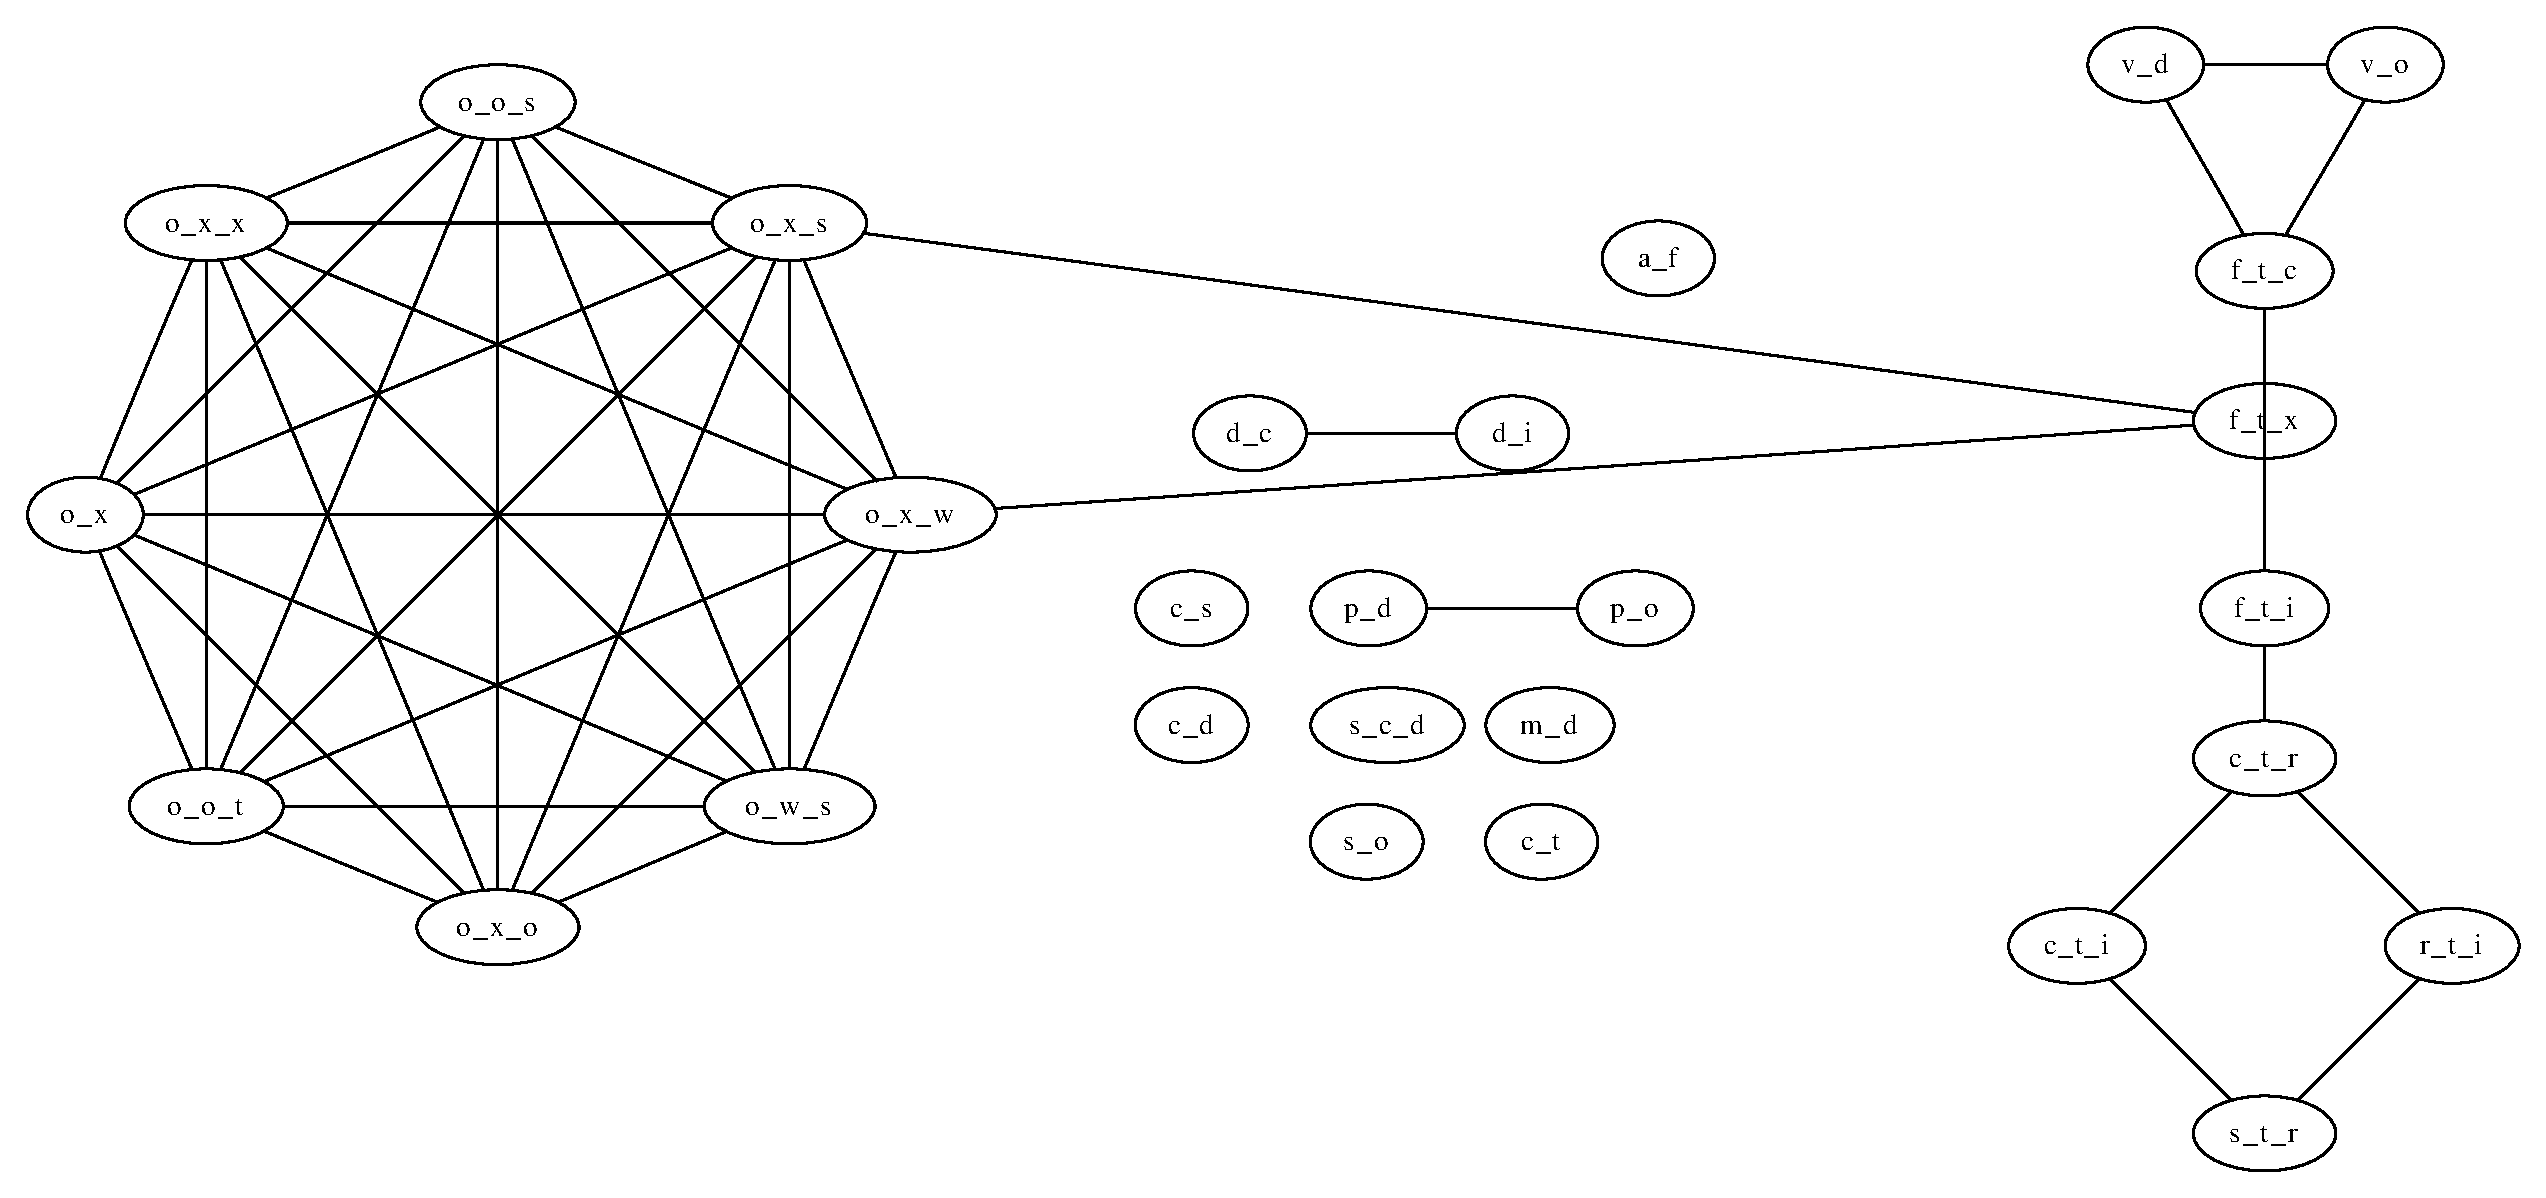
\includegraphics[width=0.45\textwidth]{images/experiments/data/realistic/OVA1}}
    \subfigure[\dataset{OVA2}]{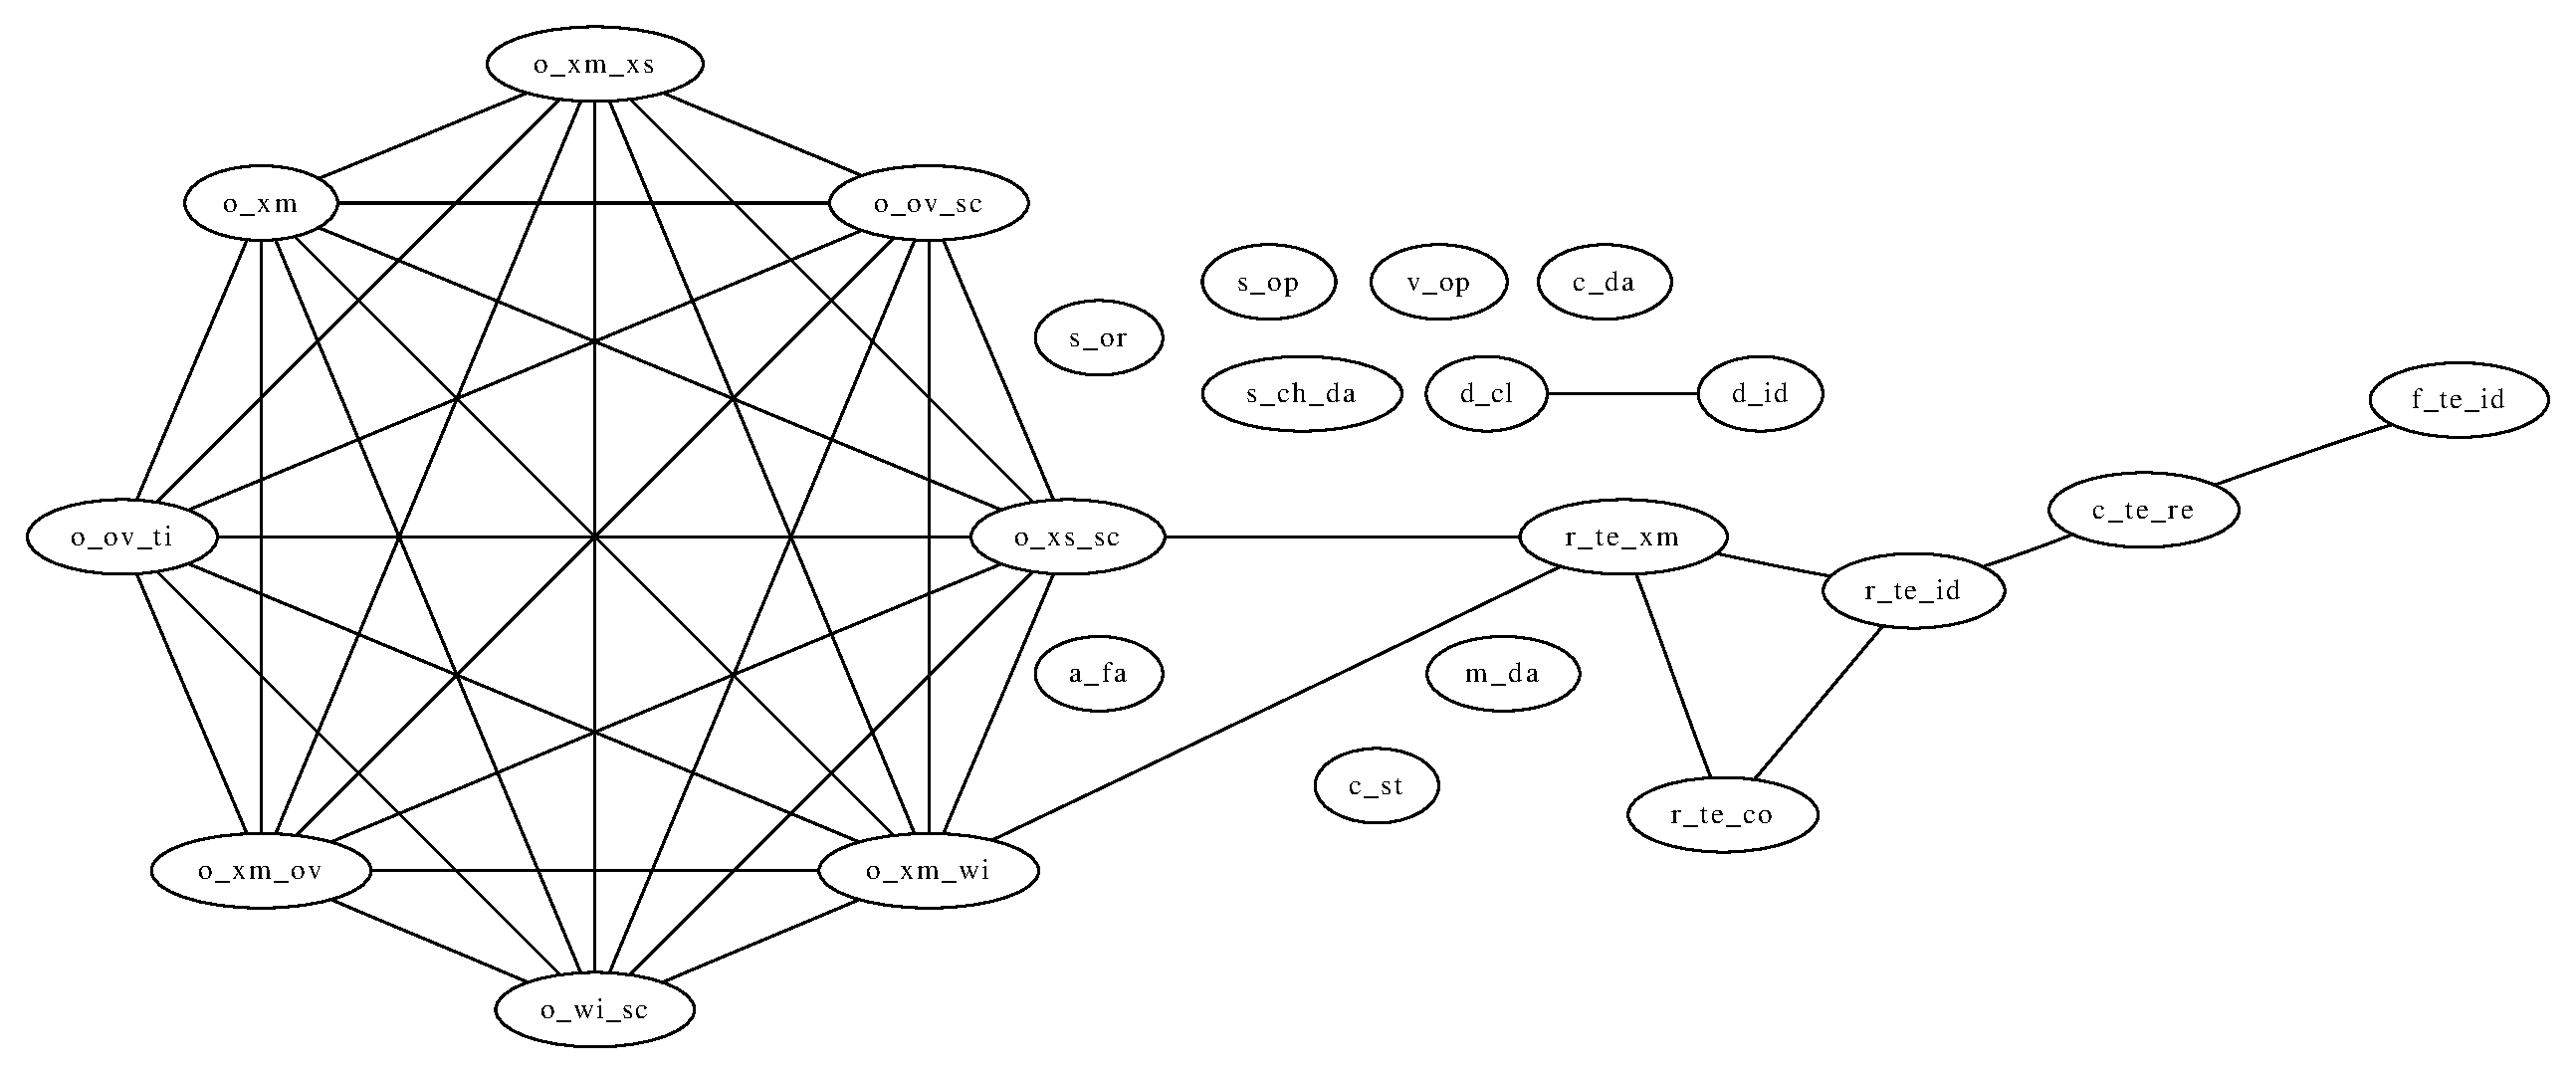
\includegraphics[width=0.45\textwidth]{images/experiments/data/realistic/OVA2}}
    \subfigure[\dataset{OVA3}]{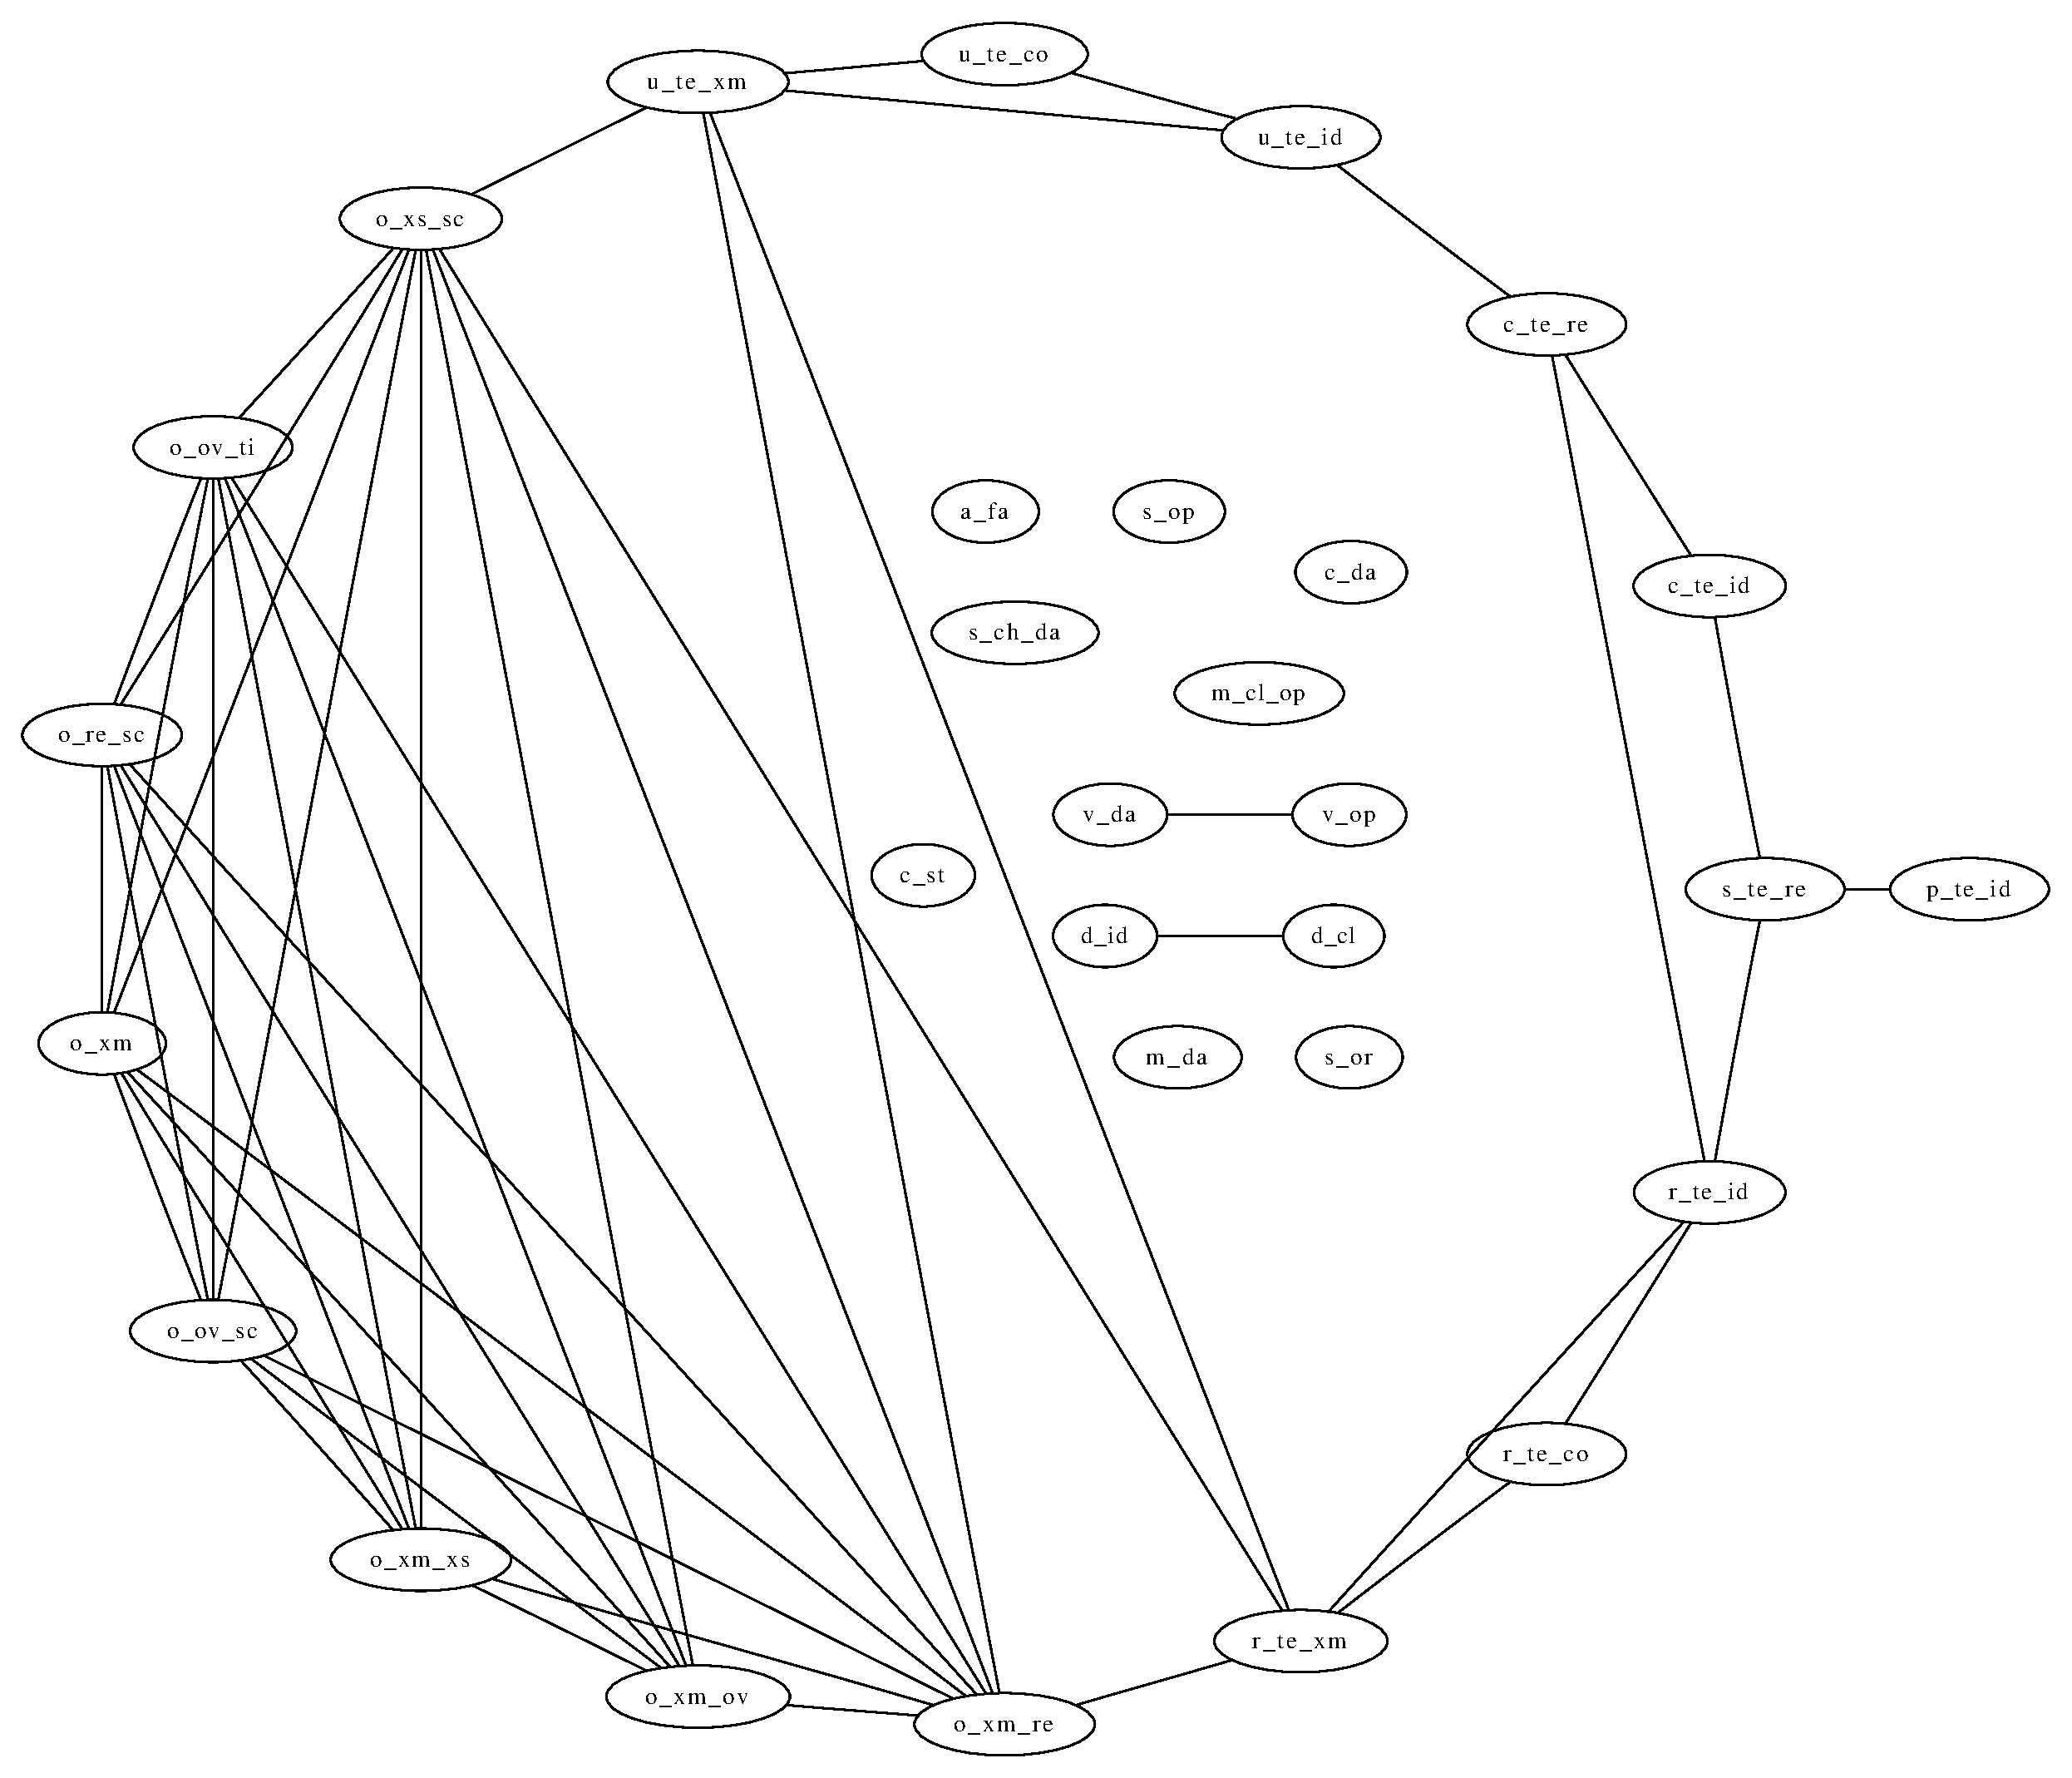
\includegraphics[width=0.45\textwidth]{images/experiments/data/realistic/OVA3}}
    \subfigure[\dataset{XMA-c}]{\includegraphics[width=0.08\textwidth]{images/experiments/data/realistic/XMA-c}}
    \subfigure[\dataset{XMA-p}]{\includegraphics[width=0.08\textwidth]{images/experiments/data/realistic/XMA-p}}
    \subfigure[\dataset{XMD}]{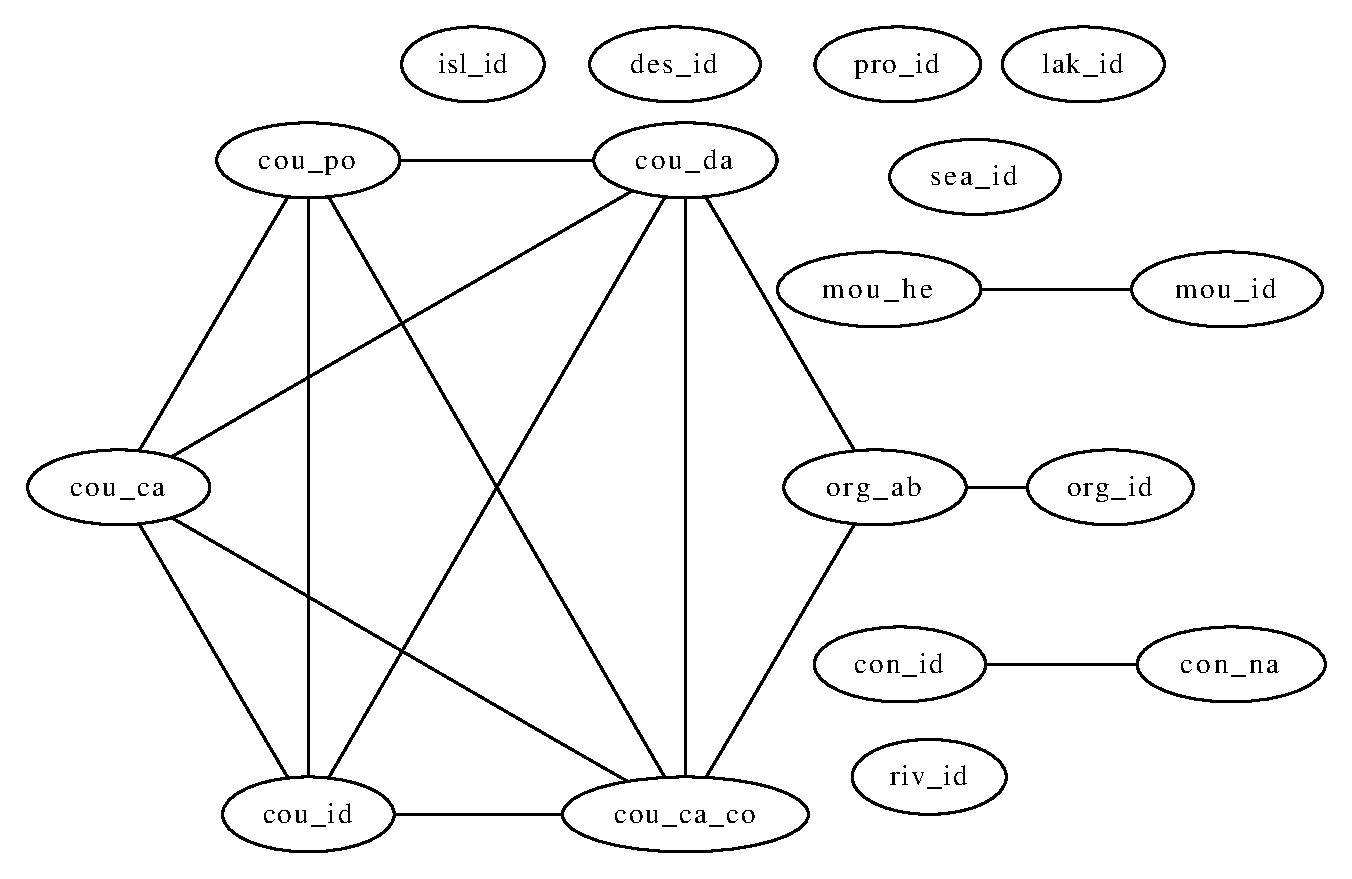
\includegraphics[width=0.45\textwidth]{images/experiments/data/realistic/XMD}}
\end{figure}

To interpret the data a little: \dataset{OVA*} sets have quite interesting and perhaps a bit challenging graphs, but are not too big. We can consider them to be the ``typical" representants.

On the other hand, the \dataset{XMA-*} sets are quite huge, but trivial: their only candidate AM will just get picked and that will be the end of the heuristic. We will see the performance of the other components of the whole system, dealing with huge data that are rather simple in the end.

Finally, the \dataset{XMD} set is quite big and at the same time has non-trivial graph representation. We should see a performance more balanced between processing and finding the ID set here.

\subsection{Realistic data with artificial attributes}
\label{realistic-converted}

We found 2 data sets to convert, \dataset{MSH} and \dataset{NTH}. Unfortunately, the same problem with disclosure as in the previous case applies here. None of these sets had any attributes before the conversion. Their summary is the Table \ref{table-experiments-data-converted}, their graphs can be seen in Figure \ref{image-experiments-data-converted}.

TODO schemas?

To address the conversion: in the case of \dataset{MSH} we found 2 elements with values looking suspiciously like a key of the records contained in the file, and converted them to be attributes of these records using a simple XSL transformation. In the case of \dataset{NTH} we converted all the values in sub-elements of the record elements to be the attributes of the records.

Why is this useful at all? Recall TODO link, where we said that ID attributes are a special case of XML keys. We can use this approach then to find XML keys: convert some suspicious data into attributes, find the optimal ID set and then create XML key based on this ID set.

\begin{table}
  \caption{List of realistic test data files with converted attributes}
  \bigskip
  \label{table-experiments-data-converted}
  \centering
  \begin{tabular}{l | r | c | c | l}
  	Name  & Size [kb] & $|V|$ & $|E|$ & Optimum \\
  	\hline
  	\dataset{MSH}  & 3 100.5 & 1 & 0 & 0.5416472778036296 \\
  	\dataset{NTH}  & 2 523.5 & 5 & 7 & 0.057918595422124436 \\
  \end{tabular}
\end{table}

\begin{figure}
  \caption{Realistic data with converted attributes}
  \label{image-experiments-data-converted}
  \centering
    \subfigure[\dataset{MSH}]{\includegraphics[width=0.08\textwidth]{images/experiments/data/converted/MSH}}
    \subfigure[\dataset{NTH}]{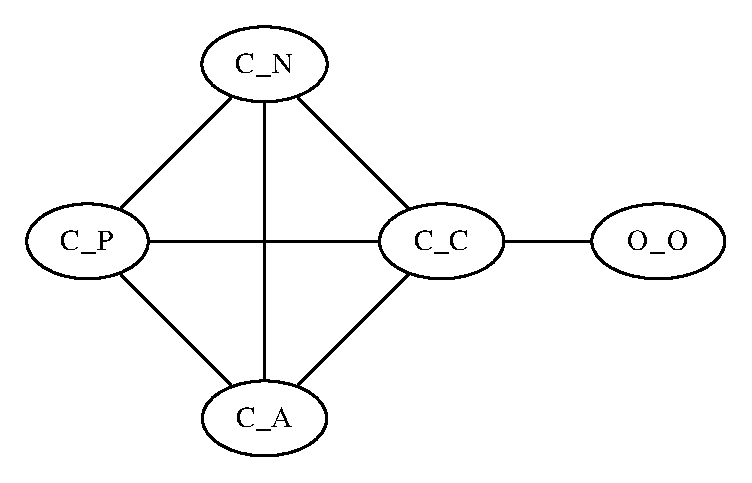
\includegraphics[width=0.45\textwidth]{images/experiments/data/converted/NTH}}
\end{figure}

Again to do a little interpretation: in the case of \dataset{MSH} we created 2 attributes, of which only one constituted a candidate AM. This is then the case similar to \dataset{XMA-*} sets: quite large data, yet only one trivial ID attribute to be found.

In the case of \dataset{NTH} we introduced more attributes, 8 to be precise. Out of them 5 proved to be candidate AMs, with 7 edges constraining them. This means we have quite a big set with relatively simple work to be done by the heuristics. This is about the change.

\subsection{Artificial data}

As soon as we started experimenting with the data coming from the real world, it was obvious that they present no real challenge to our heuristics. After we build the model, we get the most complex graphs of some 31 vertices and 47 edges (see Table \ref{table-experiments-data-realistic}). We needed to create data that would really put pressure on our heuristics, put them to a real test. Our solutions is to approach from the other side: in the end, we will be solving the equivalent of IS problem on a graph created from XML data. Why not create the XML data to contain a more complex graph in the first place? What if we could specify how many vertices and edges we want, and get the according XML?

This is actually simple. Consider the following excerpt from an XML file:

\begin{scriptsize}
\begin{verbatim}
<graph>
  <vertex0 attr="-2968876296119015800"/>
  <vertex1 attr="1729745997570096518"/>
  <vertex2 attr="-9020549659620928934"/>
  ...
  <vertex99 attr="-7545982394508643394"/>

  <vertex82 attr="0"/><vertex21 attr="0"/>
  <vertex64 attr="1"/><vertex21 attr="1"/>
  <vertex44 attr="2"/><vertex2 attr="2"/>
  ...
  <vertex96 attr="99"/><vertex40 attr="99"/>
</graph>
\end{verbatim}
\end{scriptsize}

We want to create a graph with around $v$ vertices and $e$ edges. First, we introduce $v$ elements with names \texttt{vertex0} - \texttt{vertex\{V-1\}}. To constitute an AM, they need an attribute \texttt{attr}, but with large enough random values, so that these values won't conflict with any others. Second, for each of the $e$ edges we pick two \texttt{vertex*} elements at random, and give them the same value of their \texttt{attr}. This will ensure they cannot share the same ID set, thus effectively creating the edge in the graph representation.

The pseudocode for this is in Listing \ref{listing-random-data}.

\begin{algorithm}
\caption{Random XML data creation}
\label{listing-random-data}
\begin{algorithmic}
\REQUIRE $v$ requested number of vertices
\REQUIRE $e$ requested number of edges
\ENSURE XML file content
\PRINT \texttt{<graph>}
\FOR{$i = 1 \to |V|$}
	\STATE $R \gets RANDOM$
	\PRINT \texttt{<vertex\textit{i} attr="\textit{R}">}
\ENDFOR
\FOR{$i = 1 \to |E|$}
	\STATE $v1 \gets RANDOM(|V|)$
	\STATE $v2 \gets RANDOM(|V|)$
	\PRINT \texttt{<vertex\textit{v1} attr="\textit{i}"> <vertex\textit{v2} attr="\textit{i}">}
\ENDFOR
\PRINT \texttt{</graph>}
\RETURN
\end{algorithmic}
\end{algorithm}

With this process in place we can create as much data as we wish with any combination of $v$ and $e$ we want.

There is one interesting characteristic that can describe random graphs like this, and that is the \textit{density}. This can be defined in various ways, we will use two different interpretations for a while. The first is $\frac{|E|}{|V|}$, that is, how many edges are there for one vertex (multiplied by 2 we'd get the average degree of the vertices). The second, perhaps more interesting is $\frac{|E|}{E_{max}}$, where $E_{max} = \frac{|V|.(|V|-1)}{2}$. This is the density as the ratio of edges that are to all edges that could be in a complete graph with $|V|$ vertices.

We have created 3 sets to use in experiments along with the realistic and converted sets, these are called \dataset{100-100}, \dataset{100-200} and \dataset{100-1000}. Note that the name is always in the form $v-e$.\\

All of the experimental data sets mentioned so far, realistic, converted and artificial alike will be referred to as \textit{official test data (sets)}.\\

Also, we will need data of comparably similar characteristics but varying size, to study the effects of size on the run times of experiments. For this reason we created 11 more sets, from \dataset{0-0} as the trivial one to \dataset{100-500} as the biggest one. From now on, these will be referred to as \textit{sized test data (sets)}. We wanted to keep density the same among these sets, and we picked the $\frac{|E|}{E_{max}}$ density interpretation for this.

TODO this is on the DVD.

The summary is the Table \ref{table-experiments-data-artificial} and Table \ref{table-experiments-data-artificial-size}, these tables contain 2 new columns: values of density in both interpretations we introduced. Some graphs can be seen in Figure \ref{image-experiments-data-artificial}.

While studying the tables you might notice that the actual numbers $|V|$ and $|E|$ do not match to the $v$ and $e$ in the names of the sets. This is because how the random generation algorithm works: it might pick the same edge twice, which will automatically render it unsuitable for the ID set (proof is homework). % TODO too much?:)
Because of the so-called Birthday paradox, % TODO link
this will happen more with higher $e$.

\begin{table}
  \caption{List of artificial test data files}
  \bigskip
  \label{table-experiments-data-artificial}
  \centering
  \begin{tabular}{l | r | c | c | c | c | l}
  	Name  & Size [kb] & $|V|$ & $|E|$ & $\frac{|E|}{|V|}$ & $\frac{|E|}{E_{max}}$ & Optimum \\
  	\hline
  	\dataset{100-100}  & 8.4  & 99 & 95  & 0.95 & 0.02 & 0.836666666666667 \\
  	\dataset{100-200}  & 13.0 & 96 & 174 & 1.81 & 0.04 & 0.726000000000000 \\
    \dataset{100-1000} & 49.5 & 93 & 754 & 8.11 & 0.16 & 0.380952380952381 \\
  \end{tabular}
\end{table}

\begin{table}
  \caption{List of ``sized" artificial test data files}
  \bigskip
  \label{table-experiments-data-artificial-size}
  \centering
  \begin{tabular}{l | r | c | c | c | c | l}
	  Name  & Size [kb] & $|V|$ & $|E|$ & $\frac{|E|}{|V|}$ & $\frac{|E|}{E_{max}}$ & Optimum \\
  	\hline
  	\dataset{0-0}     & 0.2  & 0  & 0   & -    & -    & 0.0                \\
  	\dataset{10-5}    & 0.6  & 10 & 5   & 0.50 & 0.11 & 0.8500000000000002 \\
    \dataset{20-20}   & 1.7  & 18 & 13  & 0.72 & 0.08 & 0.7166666666666669 \\
    \dataset{30-45}   & 3.1  & 29 & 43  & 1.48 & 0.11 & 0.7083333333333334 \\
  	\dataset{40-80}   & 5.1  & 39 & 72  & 1.85 & 0.10 & 0.6950000000000002 \\
  	\dataset{50-125}  & 7.5  & 48 & 111 & 2.31 & 0.10 & 0.6566666666666666 \\
  	\dataset{60-180}  & 10.4 & 58 & 157 & 2.71 & 0.09 & 0.6214285714285716 \\
  	\dataset{70-245}  & 13.8 & 67 & 205 & 3.06 & 0.09 & 0.5982142857142856 \\
  	\dataset{80-320}  & 17.6 & 76 & 261 & 3.43 & 0.09 & 0.5791666666666667 \\
  	\dataset{90-405}  & 21.9 & 86 & 352 & 4.09 & 0.10 & 0.528888888888889  \\
  	\dataset{100-500} & 26.7 & 91 & 388 & 4.26 & 0.09 & 0.4981818181818182 \\
  \end{tabular}
\end{table}

\begin{figure}
  \caption{Artificial data}
  \label{image-experiments-data-artificial}
  \centering
  	\subfigure[\dataset{48-80}]{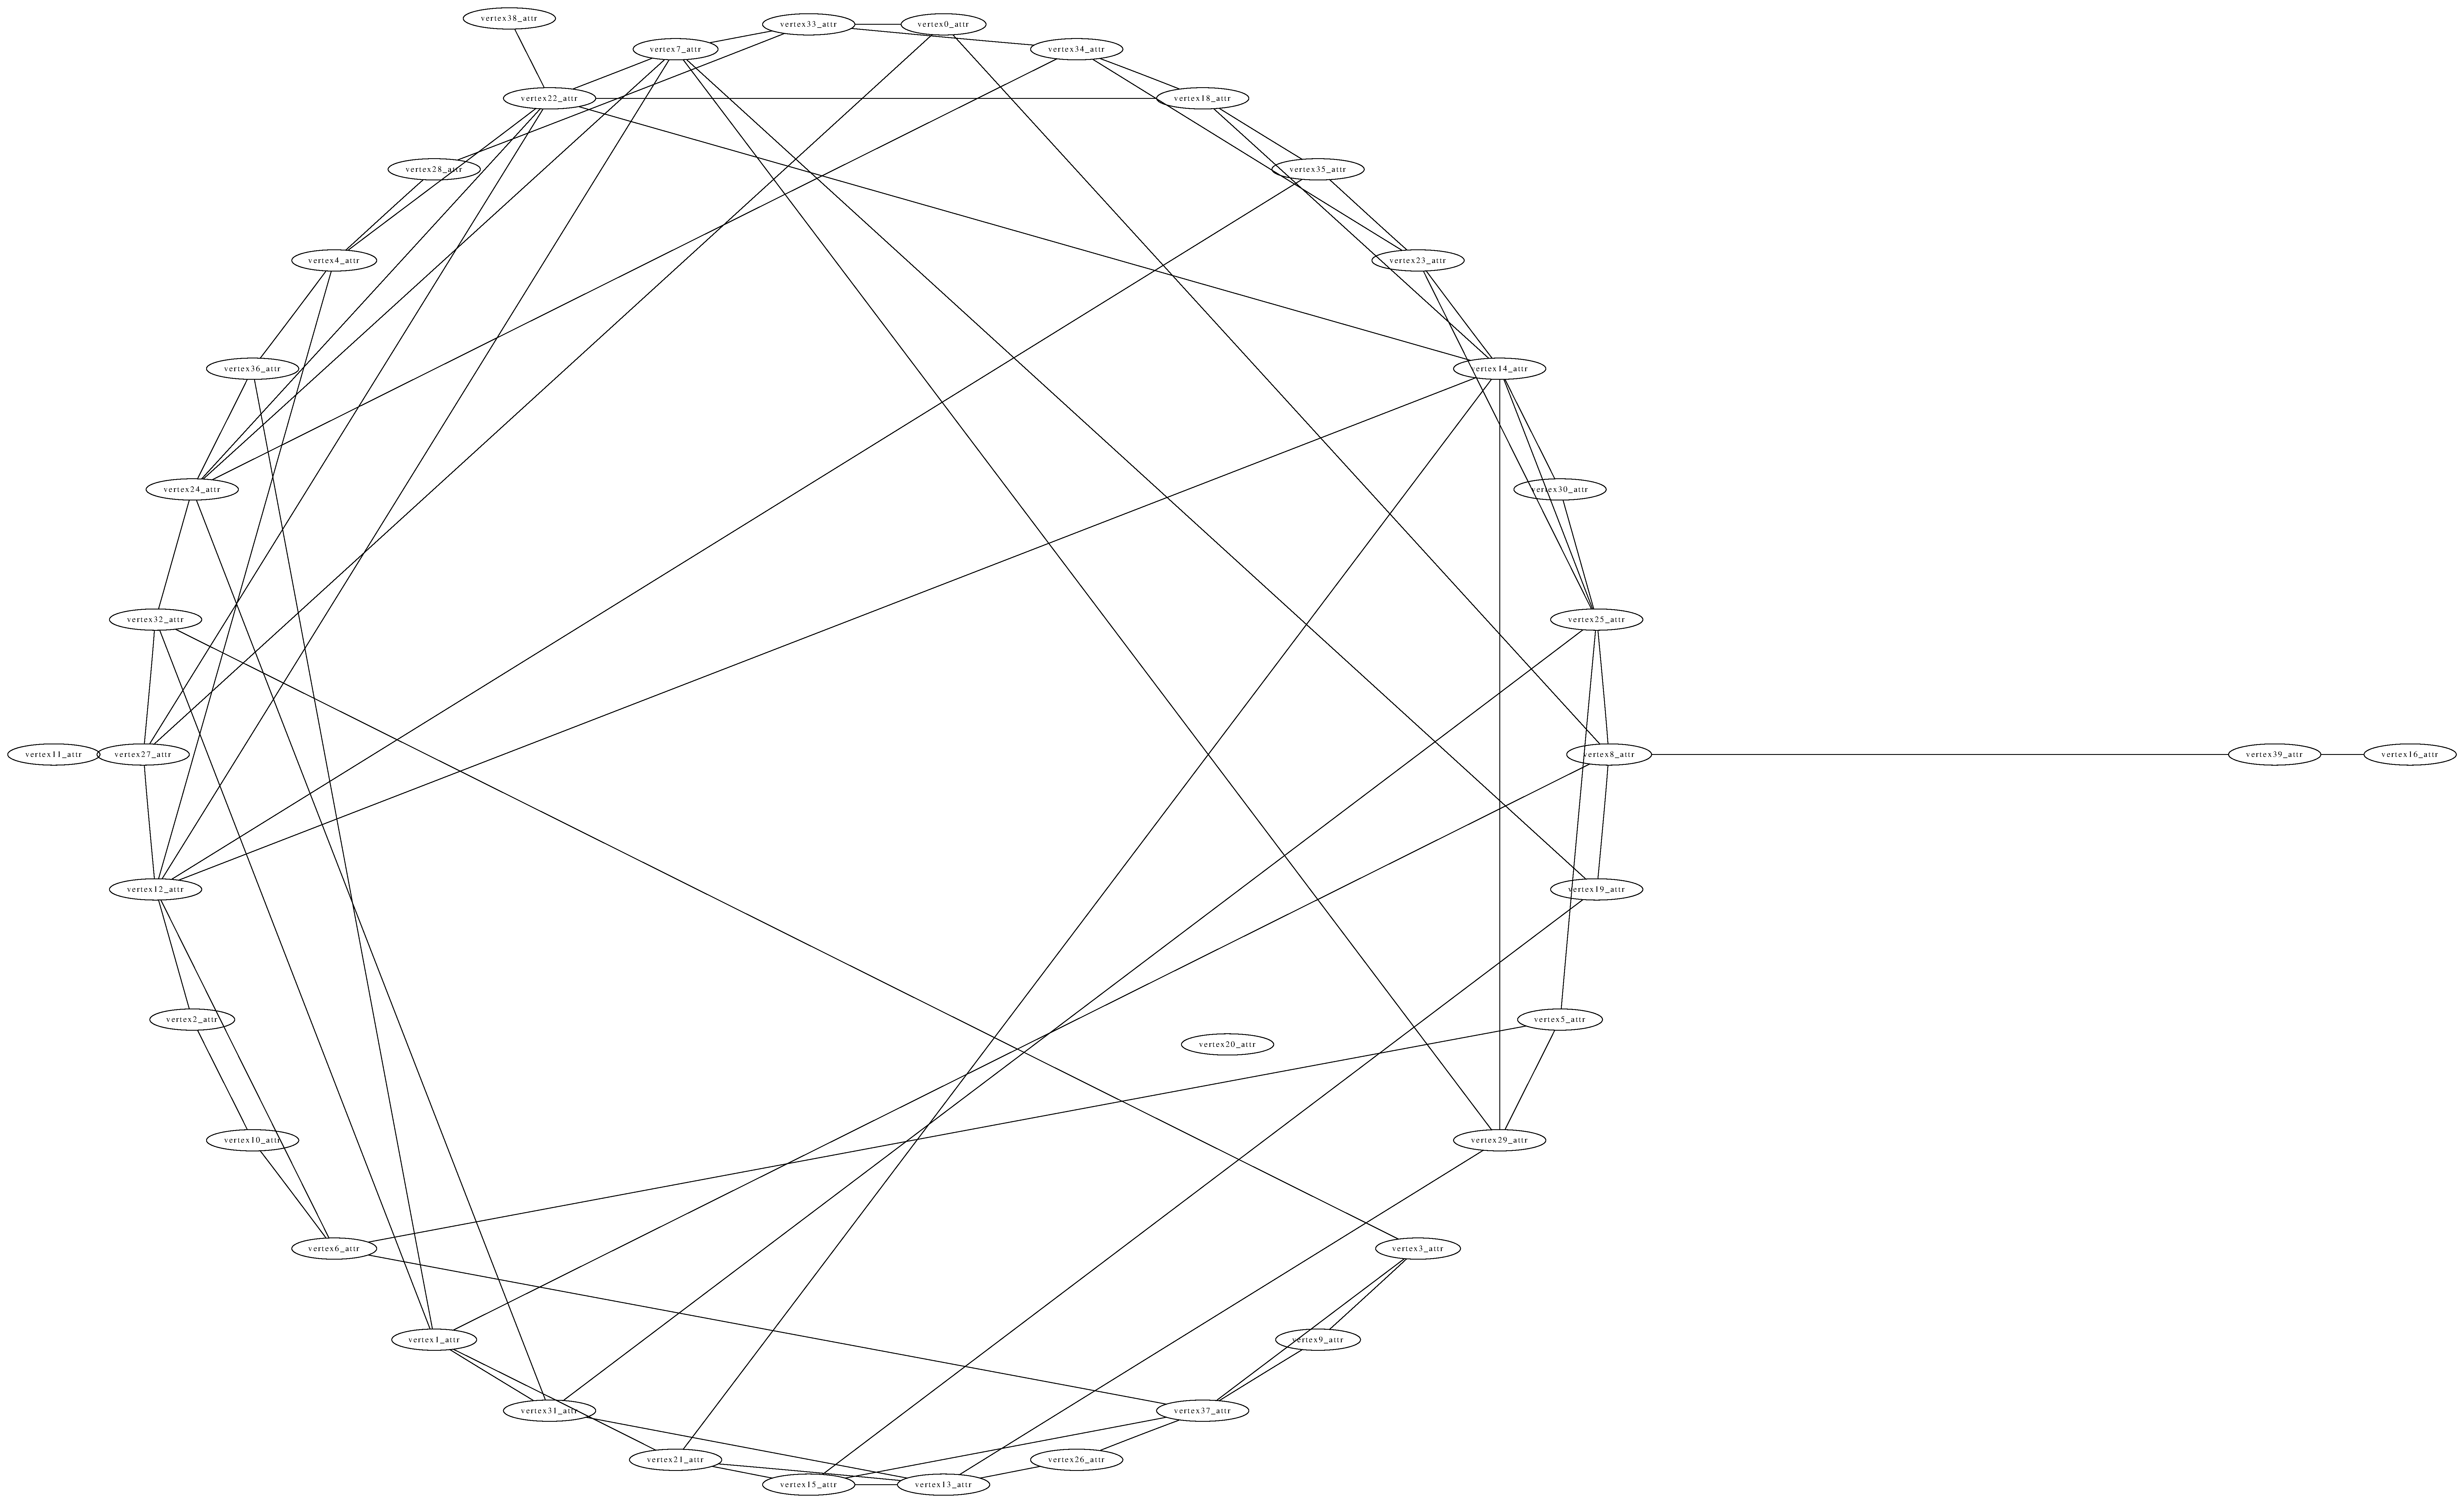
\includegraphics[width=\textwidth]{images/experiments/data/artificial/size/40-80}}
	\subfigure[\dataset{70-245}]{
\includegraphics[width=\textwidth]{images/experiments/data/artificial/size/70-245-fixed}}
\end{figure}

To interpret Tables \ref{table-experiments-data-artificial} and \ref{table-experiments-data-artificial-size}: we get 3 sets of different sizes and densities in the first one, which should work very nice with our heuristics. The $|V|$ and $|E|$ numbers are orders of magnitude higher than with any realistic (or converted) data set we are using, and this will put real stress on the heuristics, as we shall see in the next section.

In the second table we aimed for the $\frac{|E|}{E_{max}}$ density of $0.1 = 10\%$, and we can see that this was quite nicely achieved. There is an interesting observation to be made here: the optimum is steadily decreasing with the increasing overall graph size. This intuitively suggests that the maximal quality theoretically achievable has to do with the $\frac{|E|}{|V|}$ density, not with the one we fixed. Exploration of this phenomenon is among the possibilities of future work of this thesis.

\section{Experimental Setup}

As was mentioned before, we will be using an extension to the jInfer framework called \jmodule{IDSetSearch}. Please see appendices \ref{appendix-jInfer} and \ref{appendix-iss} for more detailed information on these two pieces of software.\\

We now have to define a few notions before moving forward to the description of our experiments.

\begin{define}[Experiment parameters]
	\label{define-experiment-params}
	\textit{Experiment parameters} are the following.
	\begin{itemize}
		\item All the parameters in all the heuristics.
		\item The specific way in which the heuristics are chained.
		\item Parameters $\alpha$ and $\beta$ in the weight (quality) measurement.
		\item Initial pool size.
		\item The termination criteria.
		\item The input XML file.
		\item Known optimum for this file and $\alpha$, $\beta$.
	\end{itemize}
\end{define}

\begin{define}[Experiment(al) configuration]
	\label{define-experiment-config}
	An \textit{experiment instance}, or \textit{configuration}, is one specific setting of all (experiment) parameters.
\end{define}

\begin{define}[Experiment(al) set]
	\label{define-experiment-set}
	One or more experiment configurations, regardless whether their parameters differ, constitute an \textit{experimental set}.
\end{define}

\subsection{Grammar and Model Creation}

TODO link BasicIGG to see how we get IG

TODO describe how we get the model

\subsection{Hardware and Software}

We will be using two different machines to run the experiments. Every experimental result will have explicitly stated the machine it was performed on, and we shall make sure to run different experiments that can benefit from side-by-side comparison on the same machine.

\subsubsection{Quad Core Machine}

\begin{verbatim}
Intel Core 2 Quad processor @ 2.83 GHz
8 GB DDR2 RAM
Windows 7 SP1 64bit
TODO
TODO
GLPK version TODO
\end{verbatim}

\subsubsection{Dual Core Machine}

\begin{verbatim}
Intel Core 2 Duo processor @ 2.33 GHz
4 GB DDR2 RAM
Windows 7 SP1 64bit
Java SE Runtime Environment (build 1.6.0_26-b03)
Java HotSpot 32-Bit Client VM (build 20.1-b02)
GLPK version 4.45 (Cygwin)
GLPK version 4.34 (native)
\end{verbatim}

\subsection{Methodology}

It is impossible to completely shield an experiment from the influence of the environment, but we should try our best. First of all, NetBeans running the experiments is the only relevant program running in the system at that time, as far as this is possible. Unfortunately, the NetBeans itself is quite a large environment with a life on its own, and we would most certainly get more reliable results, if we could run our experiments outside it. This improvement is left for the future work.

Also, every experimental configuration is run 50 times in hope that the effects of any events adversely affecting our results (e.g. OS deciding to run some house cleaning) will be averaged out. Whenever possible, we will always be using boxplots instead of a simple average (or average and variance) to present results of these multiple runs. % TODO discuss caches and the order in which we run the experiments in one set?

\subsection{Measuring the time}

TODO

\subsection{Obtaining the results}

Every run of an experiment produces a trace such as the one presented and commented on in Appendix \ref{appendix-trace}. We can get all the information relevant to that experiment run from this trace alone. An experimental set will produce a number of these traces and store them in plain text files in a folder. Parsing these files to aggregate and collate them might be a tedious task even using tools like \texttt{sed} and \texttt{grep}, so some of the experiment sets directly output tabular data in format recognized by GnuPlot, which we use to plot charts found in this work.

TODO explain boxplots, how to read them

\section{Experimental Results}

\subsection{Grammar and model generation}

%         NB class GrammarModelTiming

The first experiment set will try to establish how long it takes to extract the IG % TODO IG -> nomenclature
from the input XML file and how long does it take to create the AM model from this IG. For now, we will not be running or measuring any heuristics.

\begin{center}
\bigskip
\begin{tabular}{| l | l |}
  \hline
  \hline
  Machine           & Dual Core \\
  Input data        & all official and sized test data sets \\
  Iterations        & 50 \\
  Pool size         & not applicable \\
  $\alpha$, $\beta$ & not applicable \\
  \hline
\end{tabular}
\bigskip
\end{center}

The experimental set will contain $50 * (11 + 11) = 1100$ configurations: 50 iterations for 11 test data sets plus 11 sized test data sets. There will be no CHs or IHs. We will be gathering the timing data for IG extraction and model generation in GnuPlot format.

\begin{table}
  \caption{Grammar Extraction and Model Creation Times}
  \bigskip
  \label{table-experiments-grammar-model-timing}
  \centering
  \begin{tabular}{l || l | l || l | l || l | l}
    Data set & GE & GE & MC & MC & Tot & Tot \\
     & avg [ms] & stdev & avg [ms] & stdev & avg [ms] & stdev \\
    \hline
    \dataset{OVA1}     & < 10 & - & < 10 & - & < 10 & - \\
    \dataset{OVA2}     & < 10 & - & < 10 & - & < 10 & - \\
    \dataset{OVA3}     & 42.94 & 19.8509 & 60.92 & 27.0848 & 103.86	& 31.6911 \\
    \dataset{XMA-c}    & 140.32 &	33.2618 &	90.24 &	45.8803 & 230.56 & 56.2633 \\
	\dataset{XMA-p}    & 7518.82 &	922.8882 &	10135.46 &	502.8997 & 17654.28	& 1353.8794 \\
	\dataset{XMD}      & 979.18 &	307.1760 &	563.04 & 341.4697 & 1542.22	& 134.6883 \\
	\dataset{MSH}      & 570.24 &	167.1119 &	225.48 &	90.6775 & 795.72 & 161.8340 \\ 
	\dataset{NTH}      & 328.36 & 118.3766 &	1074.9 &	155.5604 & 1403.26 & 137.8695 \\
	\dataset{100-100}  & < 10 & - & < 10 & - & < 10 & - \\
	\dataset{100-200}  & < 10 & - & < 10 & - & < 10 & - \\
	\dataset{100-1000} & 18.34 & 10.2372 & 18.84 & 1.0373 & 37.18 & 9.9338 \\
	\dataset{0-0}      & < 10 & - & < 10 & - & < 10 & - \\
	\dataset{10-5}     & < 10 & - & < 10 & - & < 10 & - \\
	\dataset{20-20}    & < 10 & - & < 10 & - & < 10 & - \\
	\dataset{30-45}    & < 10 & - & < 10 & - & < 10 & - \\
	\dataset{40-80}    & < 10 & - & < 10 & - & < 10 & - \\
	\dataset{50-125}   & < 10 & - & < 10 & - & < 10 & - \\
	\dataset{60-180}   & < 10 & - & < 10 & - & < 10 & - \\
	\dataset{70-245}   & < 10 & - & < 10 & - & < 10 & - \\
	\dataset{80-320}   & < 10 & - & < 10 & - & 12.48 & 8.3574 \\
	\dataset{90-405}   & < 10 & - & < 10 & - & 15.88 & 10.3778 \\
	\dataset{100-500}  & < 10 & - & < 10 & - & 18.74 &	8.8889 \\
  \end{tabular}
\end{table}

Results are in Table \ref{table-experiments-grammar-model-timing}. We are presenting the average grammar extraction (GE) times and their standard deviation, the same for model creation (MC) and total (sum of these two, Tot) times. For many data sets the average time is less than 10 ms: this is not enough to be precise and we don't calculate the standard deviation in these cases.

We can see from the results that for most data sets their model can easily be created under around one second, only in case of the biggest set \dataset{XMA-p} (13 MB) this takes some 17 seconds. We can conclude that grammar and model creation times are not a bottleneck for now. Heuristics run times will be order of magnitude higher.

\subsubsection{GLPK interface timing}

%         NB class GlpkInterfaceTiming

A related problem is how long it takes to create input for GLPK and then parse its results. We will use the same test data sets as in the previous case, but now we will gather times needed to communicate with GLPK.

\begin{table}
  \caption{GLPK Interface Times}
  \bigskip
  \label{table-experiments-glpk-timing}
  \centering
  \begin{tabular}{l || l | l || l | l || l | l}
	Data set & IC & IC & OP & OP & Tot & Tot \\
     & avg [ms] & stdev & avg [ms] & stdev & avg [ms] & stdev \\
	\hline
	\dataset{OVA1} & 36.46 & 66.8517 & 49.8 & 114.0687 & 86.26 & 150.1044 \\
	\dataset{OVA2} & 39.52 & 75.8210 & 48.8 & 102.4484 & 88.32 & 154.9596 \\
	\dataset{OVA3} & 34.1 & 74.1838 & 38.62 & 89.3772 & 72.72 & 134.7295 \\
	\dataset{XMA-c} & 40.88 & 88.6632 & 33.84 & 65.8636 & 74.72 & 127.7338 \\
	\dataset{XMA-p} & 36.54 & 70.7436 & 49.24 & 101.2412 & 85.78 & 145.2092 \\
	\dataset{XMD} & 37.98 & 69.2719 & 32.88 & 70.2173 & 70.86 & 114.6692 \\
	\dataset{MSH} & 40.42 & 91.9885 & 36.52 & 72.1018 & 76.94 & 138.6198 \\
	\dataset{NTH} & 36.02 & 66.3403 & 38.06 & 88.8244 & 74.08 & 128.9974 \\
	\dataset{100-100} & 46.5 & 103.3929 & 46.92 & 89.7049 & 93.42 & 158.7267 \\
	\dataset{100-200} & 42.34 & 96.1204 & 38.22 & 90.0284 & 80.56 & 152.6534 \\
	\dataset{100-1000} & 32.92 & 64.4534 & 42.1 & 89.4546 & 75.02 & 127.8541 \\
	\dataset{0-0} & 46.8 & 123.5183 & 46.92 & 102.2601 & 93.72 & 181.5228 \\
	\dataset{10-5} & 40.06 & 75.7370 & 40.1 & 72.4851 & 80.16 & 126.7135 \\
	\dataset{20-20} & 33.72 & 70.7263 & 34.1 & 66.2781 & 67.82 & 116.3783 \\
	\dataset{30-45} & 38.26 & 71.7549 & 45.94 & 110.1284 & 84.2 & 155.7594 \\
	\dataset{40-80} & 37.06 & 67.0024 & 49.26 & 106.3185 & 86.32 & 144.9918 \\
	\dataset{50-125} & 50.44 & 101.9162 & 84.76 & 364.7350 & 135.2 & 378.7835 \\
	\dataset{60-180} & 38.38 & 89.3379 & 42.54 & 94.3742 & 80.92 & 149.6049 \\
	\dataset{70-245} & 41.5 & 93.2951 & 40.3 & 93.4858 & 81.8 & 149.6797 \\
	\dataset{80-320} & 51.92 & 121.9812 & 47.98 & 96.0904 & 99.9 & 171.4617 \\
	\dataset{90-405} & 40.5 & 91.5373 & 36.46 & 88.5099 & 76.96 & 144.2890 \\
	\dataset{100-500} & 37.82 & 85.7571 & 43.4 & 90.3257 & 81.22 & 141.9103 \\
  \end{tabular}
\end{table}

Results are in table \ref{table-experiments-glpk-timing}. For each data set there are the times of (GLPK) input creation (IC) - average and standard deviation, then the same for output parsing (OP) and total (Tot).

Interestingly enough, in most cases the times to create an input for GLPK and then to parse its output are very similar. Also, for sized test data sets it is interesting to note that even though the $|V|$ and $|E|$ counts are increasing, the times remain almost the same. This probably due to the fact that IC and OP times include the I/O when writing to a file for GLPK or reading the file it produced, and these times are probably the most relevant.

\subsection{GLPK: native vs. Cygwin}

%         NB class TimeQuality
%         NB class TimeTillOptimum

In this experiment we will try to remove one of the variables out of the equation: that is the effect of different versions of GLPK on the overall results. The rationale is this: on Windows systems, the two most accessible ways to install GLPK are via a binary distribution, % TODO link
or via Cygwin as one of its packages.

If we find out which of these Cygwin version is better, we will be using it exclusively knowing this should not affect any other aspect of our experiments. We might also find that there is no relevant difference, which would be and interesting finding, too.

Apart from comparing different versions, we shall see how the pure GLPK approach behaves. The first part of this experiment will be limiting the run time, thus making it an instance of \heu{Truncated branch \& bound}. In this case we will see the dependency between the run time and the quality achieved in it. In the second time we will let GLPK run until optimum is found. We shall see the dependency between input size and run time needed to achieve the optimum.

\begin{center}
\bigskip
\begin{tabular}{| l | l |}
  \hline
  \hline
  Machine           & Dual Core \\
  Input data        & \dataset{100-500} \\
  Iterations        & 50 \\
  Pool size         & 1 \\
  $\alpha$, $\beta$ & $1$, $1$ \\
  \hline
\end{tabular}
\bigskip
\end{center}

Our experimental set will contain 500 experimental configurations for each of these two GLPK version. Every configuration will use \heu{Glpk} CH set to a time limit from 1 to 46 seconds with increments of 5, meaning 10 settings * 50 iterations = 500 configurations in total (see Listing \ref{listing-experiment-glpk-native-vs-cygwin-1}). There will be no improvement heuristic. The only data we gather in the GnuPlot file are the final qualities (weights). The data set used is \dataset{100-500} as the biggest one in sized test data.

\begin{algorithm}
\caption{GLPK: native vs. Cygwin set generation 1}
\label{listing-experiment-glpk-native-vs-cygwin-1}
\begin{algorithmic}
\ENSURE experimental set $ES$
\STATE $ES \gets \emptyset$
\FOR{$i = 1 \to 50$}
	\FOR{$time = 1 \to 46$ step $5$}
    \STATE $ES \gets ES \cup {CH = \heu{Glpk}(limit = time), IH = \emptyset}$
  \ENDFOR
\ENDFOR
\RETURN $ES$
\end{algorithmic}
\end{algorithm}

\begin{figure}
  \caption{Time vs. Quality}
  \label{image-experiment-time-vs-quality}
  \centering
    \includegraphics[width=\textwidth]{images/experiments/time-vs-quality}
\end{figure}

Results are in Figure \ref{image-experiment-time-vs-quality}. They should be interpreted as follows: for each time limit from 1 to 46 seconds there are two boxplots next to each other, the left, dashed one is the native GLPK, the right, solid one is the Cygwin GLPK. This is reflected in the tics on the X (time) axis, meaning that the axis cannot be interpreted in the usual way.

We can see from the graph that even though for smaller times (1 and 6 seconds, respectively) the Cygwin GLPK is reaching better qualities with smaller variance, starting from 11 seconds the native GLPK is at least as good or better for every following time. The results are inconclusive though, it is necessary to wait for confirmation from the second part of this experiment.

\begin{center}
\bigskip
\begin{tabular}{| l | l |}
  \hline
  \hline
  Machine           & Dual Core \\
  Input data        & all sized test data sets \\
  Iterations        & 50 \\
  Pool size         & 1 \\
  $\alpha$, $\beta$ & $1$, $1$ \\
  \hline
\end{tabular}
\bigskip
\end{center}

The other way to compare the performance of these two GLPK versions is to see how long it takes them to find the optimum for a set of data of increasing size. This experimental set will contain 550 configurations for each version. Every configuration will let \heu{Glpk} CH run for unlimited time, until it finds the optimum. This will be repeated in 50 iterations for each of the 11 files from the sized test data set (see Listing \ref{listing-experiment-glpk-native-vs-cygwin-2}). There will again be no IH, the only data we will collect are the times of the CH run in each case.

\begin{algorithm}
\caption{GLPK: native vs. Cygwin set generation 2}
\label{listing-experiment-glpk-native-vs-cygwin-2}
\begin{algorithmic}
\ENSURE experimental set $ES$
\STATE $ES \gets \emptyset$
\FOR{$i = 1 \to 50$}
	\FOR{$file \in $ sized test data}
    \STATE $ES \gets ES \cup \{file, CH = \heu{Glpk}(no\:limit), IH = \emptyset\}$
  \ENDFOR
\ENDFOR
\RETURN $ES$
\end{algorithmic}
\end{algorithm}

\begin{figure}
  \caption{Time Until Optimum}
  \label{image-experiment-time-until-optimum}
  \centering
    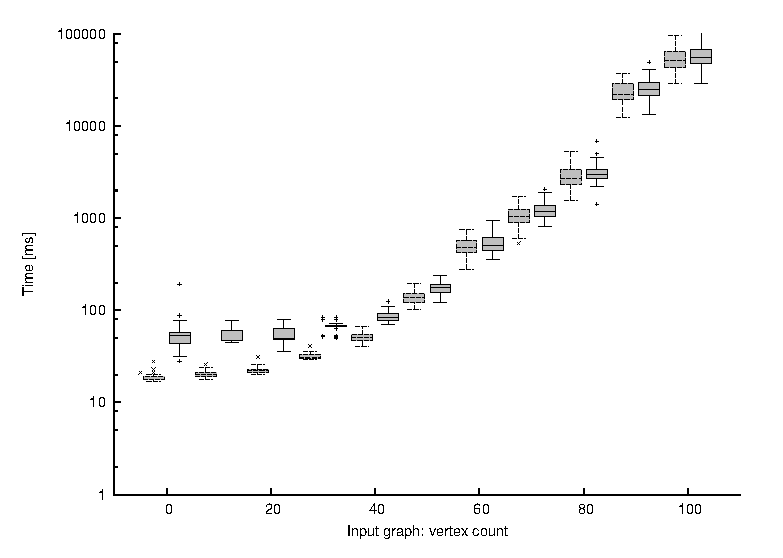
\includegraphics[width=\textwidth]{images/experiments/time-till-optimum}
\end{figure}

Results are in Figure \ref{image-experiment-time-until-optimum}, please take a note that the Y axis is in log scale. As with the previous case, the X axis cannot be interpreted in the usual way. For each data set there are two boxplots next to each other: the left one is the native GLPK, the right one is the Cygwin GLPK.

From these results it becomes clear that the native GLPK has in general shorter running times for each and every input data set than its Cygwin counterpart. This becomes less extreme with the increasing input size, which leads us to suspicion that the core parts of computation in both cases are equally powerful. Regardless of that, we shall be using the \textbf{native} GLPK for following experiments.

To conclude the first timing experiments we introduce a summary pie chart in Figure \ref{image-experiment-timing-summary}. This shows the typical distribution of times needed to find the optimum for the \dataset{OVA3} data set.

These experiments proved that for bigger data sets the times to reach the optimum might become too long. We shall attempt to find heuristics to reach the optimum faster in the following experiments.

% TODO fix this chart
\begin{figure}
  \caption{Timing Summary}
  \label{image-experiment-timing-summary}
  \centering
    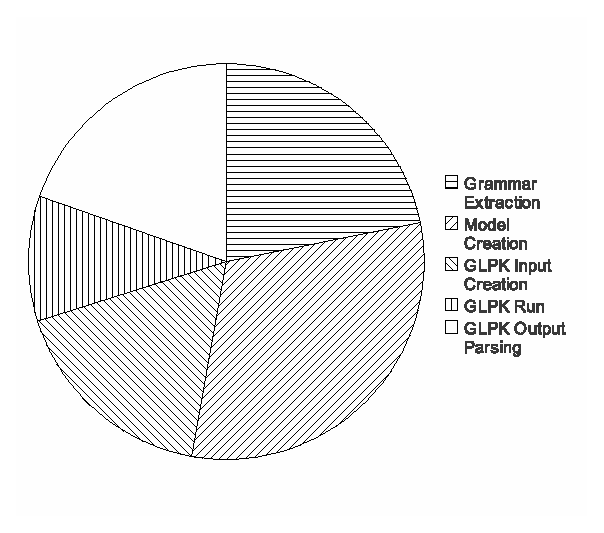
\includegraphics[width=.6\textwidth]{images/experiments/timing-pie}
\end{figure}

\subsection{\heu{Random} vs. \heu{Fuzzy} vs. \heu{FIDAX}}

%         NB class RandomVsFuzzyVsFidaxStart

Our investigation into various CHs will start by comparing \heu{FIDAX} from the original article \cite{fidax} to 2 of our trivial randomized hungry heuristics, \heu{Random} and \heu{Fuzzy}.

\begin{center}
\bigskip
\begin{tabular}{| l | l |}
  \hline
  \hline
  Machine           & Dual Core \\
  Input data set    & all official test data sets \\
  Iterations        & 50 \\
  Pool size         & 10 \\
  $\alpha$, $\beta$ & $1$, $1$ \\
  \hline
\end{tabular}
\bigskip
\end{center}

The experimental set will contain 1650 configurations in total: 3 different CHs * 11 official test data sets * 50 iterations. There will be no improvement heuristics. The pool size will be set to 10, even though \heu{FIDAX} cannot not profit from this. Listing for this can be found in \ref{listing-experiment-random-fuzzy-fidax}.

We will be gathering the running time of the CH itself and quality of the best solution found for GnuPlot.

\begin{algorithm}
\caption{\heu{Random} vs. \heu{Fuzzy} vs. \heu{FIDAX} set generation}
\label{listing-experiment-random-fuzzy-fidax}
\begin{algorithmic}
\ENSURE experimental set $ES$
\STATE $ES \gets \emptyset$
\FOR{$i = 1 \to 50$}
	\FOR{$file \in $ official test data}
    \STATE $ES \gets ES \cup \{file, CH = \heu{Random}(pool = 10), IH = \emptyset\} \cup \{file, CH = \heu{Fuzzy}(pool = 10), IH = \emptyset\} \cup \{file, CH = \heu{FIDAX}, IH = \emptyset\}$
  \ENDFOR
\ENDFOR
\RETURN $ES$
\end{algorithmic}
\end{algorithm}

\begin{figure}
  \caption{Random vs. Fuzzy vs. FIDAX - Quality}
  \label{image-experiment-random-fuzzy-fidax-quality}
  \centering
    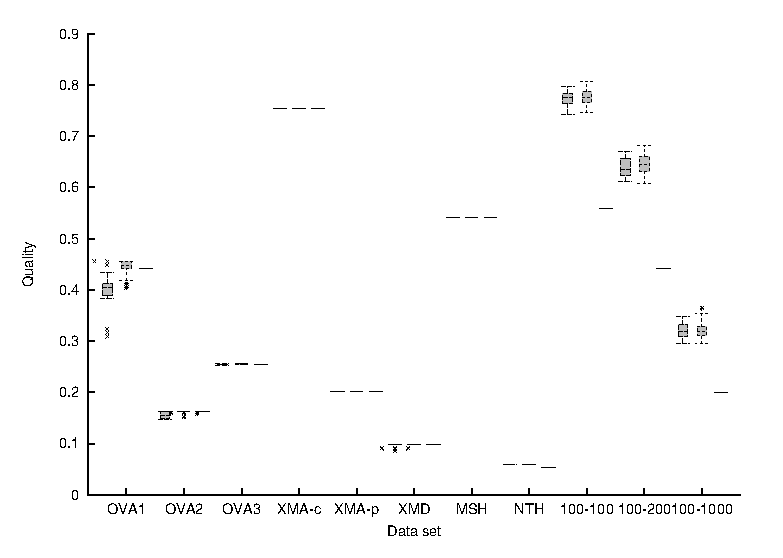
\includegraphics[width=\textwidth]{images/experiments/random-fuzzy-fidax-quality}
\end{figure}

\begin{figure}
  \caption{Random vs. Fuzzy vs. FIDAX - Time}
  \label{image-experiment-random-fuzzy-fidax-time}
  \centering
    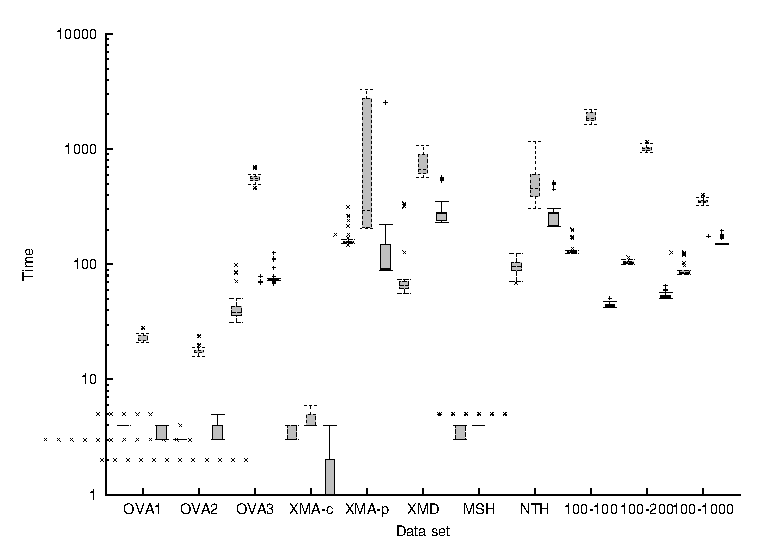
\includegraphics[width=\textwidth]{images/experiments/random-fuzzy-fidax-time}
\end{figure}

Results can be found in Figure \ref{image-experiment-random-fuzzy-fidax-quality} - qualities achieved and Figure \ref{image-experiment-random-fuzzy-fidax-time} - times spent. The Y (time) axis in the latter figure is again in log scale. For each data set there are 3 boxplots next to each other. The first, leftmost, represents \heu{Random}, second \heu{Fuzzy} and finally the third, rightmost is \heu{FIDAX}.

We can draw the following conclusions. \heu{Fuzzy} consistently finds the best solution, but it's by far the slowest of these CHs. The trivial \heu{Random} is better than \heu{FIDAX} in artificial as well as some real data.

\subsubsection{Improving \heu{FIDAX} with \heu{Hungry}}

%         NB class FidaxWithHungry

Now we shall try to answer a minor question, whether it is possible to improve \heu{FIDAX} by using \heu{Hungry} as IH. This short experiment answers that question.

\begin{center}
\bigskip
\begin{tabular}{| l | l |}
  \hline
  \hline
  Machine           & Dual Core \\
  Input data set    & all official test data sets \\
  Iterations        & 1 \\
  Pool size         & 1 \\
  $\alpha$, $\beta$ & $1$, $1$ \\
  \hline
\end{tabular}
\bigskip
\end{center}

We need a pool size of one and only a single iteration - both \heu{FIDAX} and \heu{Hungry} are deterministic. We will try all official data sets, first with empty IH, second with \heu{Hungry} as IH. We will gather the qualities in each case and see whether there is any improvement.

The experimental results are summarized in the Table \ref{table-experiments-fidax-and-hungry} and are quite surprising. As trivial a heuristic \heu{Hungry} is, it is still able to improve the ID set found by \heu{FIDAX} by as much as almost 50\% (the last row, \dataset{100-1000}).

Table \ref{table-experiments-fidax-and-hungry-idsets} lists the ID attributes found in both cases for this most extreme input, \dataset{100-1000}. Note that the content of each cell means ``attribute \texttt{attr} in element \texttt{vertexXY} should be marked as ID attribute".

\begin{table}
  \caption{Results of adding \heu{Hungry} after \heu{FIDAX}}
  \bigskip
  \label{table-experiments-fidax-and-hungry}
  \centering
  \begin{tabular}{l | l | l}
    Data set & Quality - \heu{FIDAX} & Quality - \heu{FIDAX} + \heu{Hungry} \\
    \hline
    \dataset{OVA1}     & 0.4411764705882353  & 0.4411764705882353   \\
    \dataset{OVA2}     & 0.16346153846153846 & 0.16346153846153846  \\
    \dataset{OVA3}     & 0.25482414123443264 & \textbf{0.2553715615163541}   \\
    \dataset{XMA-c}    & 0.7546666666666666	 & 0.7546666666666666   \\
    \dataset{XMA-p}    & 0.2019306150568969	 & 0.2019306150568969   \\
    \dataset{XMD}      & 0.09786094165493509 & 0.09786094165493509  \\
    \dataset{MSH}      & 0.5416472778036296	 & 0.5416472778036296   \\
    \dataset{NTH}      & 0.05259709474828076 & \textbf{0.057918595422124436} \\
    \dataset{100-100}  & 0.56	               & \textbf{0.6766666666666669}   \\
    \dataset{100-200}  & 0.44200000000000017 & \textbf{0.5980000000000003}   \\
    \dataset{100-1000} & 0.19952380952380955 & \textbf{0.29619047619047617}  \\
  \end{tabular}
\end{table}

% TODO for some reason \texttt{\textbf{vertex5}} looks only like \texttt{vertex5}
\begin{table}
  \caption{ID sets in \heu{FIDAX} versus \heu{FIDAX} + \heu{Hungry}}
  \bigskip
  \label{table-experiments-fidax-and-hungry-idsets}
  \centering
  \begin{tabular}{l | l}
  \heu{FIDAX} & \heu{FIDAX} + \heu{Hungry} \\
  \hline
                    & \texttt{\textbf{vertex5}}  \\
                    & \texttt{\textbf{vertex26}} \\
  \texttt{vertex30} & \texttt{vertex30} \\
  \texttt{vertex31} & \texttt{vertex31} \\
  \texttt{vertex32} & \texttt{vertex32} \\
  \texttt{vertex34} & \texttt{vertex34} \\
  \texttt{vertex35} & \texttt{vertex35} \\
  \texttt{vertex36} & \texttt{vertex36} \\
  \texttt{vertex37} & \texttt{vertex37} \\
  \texttt{vertex39} & \texttt{vertex39} \\
                    & \texttt{\textbf{vertex60}} \\
                    & \texttt{\textbf{vertex69}} \\
                    & \texttt{\textbf{vertex70}} \\
  \texttt{vertex74} & \texttt{vertex74} \\
  \texttt{vertex75} & \texttt{vertex75} \\
  \texttt{vertex80} & \texttt{vertex80} \\
  \end{tabular}
\end{table}

\subsection{Best standalone CH}

%         NB class BestStandaloneCH

We shall now try to find the best standalone CH, that is the CH that finds on average the best solutions when run without any IHs. We need to set a time limit for \heu{Glpk} to make it an instance of \heu{Truncated Branch \& Bound}, and we shall use 1 second. This is the smallest time limit possible for GLPK and it is still a reasonably short time, fair to other CHs.

\begin{center}
\bigskip
\begin{tabular}{| l | l |}
  \hline
  \hline
  Machine           & Quad Core \\
  Input data        & all official test data sets \\
  Iterations        & 50 \\
  Pool size         & 10 \\
  $\alpha$, $\beta$ & $1$, $1$ \\
  \hline
\end{tabular}
\bigskip
\end{center}

We will use all the official data sets, set the pool size to 10 where applicable, $\alpha$ and $\beta$ to 1. This experiment will consist of 50 iterations * 11 data sets * 6 CHs = 3300 experimental configurations. See the Listing \ref{listing-experiment-best-standalone-ch} for details. This time we are not interested in run times, only in qualities which we shall gather in a format for GnuPlot.

\begin{algorithm}
\caption{Best Standalone CH set generation}
\label{listing-experiment-best-standalone-ch}
\begin{algorithmic}
\ENSURE experimental set $ES$
\STATE $ES \gets \emptyset$
\FOR{$file \in $ official test data}
	\FOR{$i = 1 \to 50$}
    	\STATE $ES \gets ES \cup \{file, CH = \heu{Random}, IH = \emptyset\}$
    	\STATE $ES \gets ES \cup \{file, CH = \heu{Fuzzy}, IH = \emptyset\}$
    	\STATE $ES \gets ES \cup \{file, CH = \heu{Incremental}, IH = \emptyset\}$
    	\STATE $ES \gets ES \cup \{file, CH = \heu{Removal}, IH = \emptyset\}$
    	\STATE $ES \gets ES \cup \{file, CH = \heu{FIDAX}, IH = \emptyset\}$
    	\STATE $ES \gets ES \cup \{file, CH = \heu{Glpk}(limit = 1), IH = \emptyset\}$
  \ENDFOR
\ENDFOR
\RETURN $ES$
\end{algorithmic}
\end{algorithm}

For data sets \heu{XMA-c}, \heu{XMA-p}, \heu{MSH} and \heu{NTH} every CH found the optimum every time. Graphs representing the results for remaining data sets can be found in Figure \ref{image-experiments-best-standalone-ch}.

\begin{figure}
  \caption{Best Standalone CH}
  \label{image-experiments-best-standalone-ch}
  \centering
  	\subfigure[\dataset{OVA1}]{\includegraphics[width=.45\textwidth]{images/experiments/best-ch-OVA1}}
  	\subfigure[\dataset{OVA2}]{\includegraphics[width=.45\textwidth]{images/experiments/best-ch-OVA2}}
  	\subfigure[\dataset{OVA3}]{\includegraphics[width=.45\textwidth]{images/experiments/best-ch-OVA3}}
  	\subfigure[\dataset{XMD}]{\includegraphics[width=.45\textwidth]{images/experiments/best-ch-XMD}}
   	\subfigure[\dataset{100-100}]{\includegraphics[width=.45\textwidth]{images/experiments/best-ch-100-100}}
  	\subfigure[\dataset{100-200}]{\includegraphics[width=.45\textwidth]{images/experiments/best-ch-100-200}}
  	\subfigure[\dataset{100-1000}]{\includegraphics[width=.45\textwidth]{images/experiments/best-ch-100-1000}}
\end{figure}

We can see that \heu{Glpk} wins in every single case. We will start from there and try to build upon this result.

\subsection{Best IH for Glpk}

%         NB class BestIHForGlpk

The next logical step will be to try to add one IH after the best CH we have found, \heu{Glpk}. We will investigate all IHs except for \heu{RandomRemove} and \heu{RemoveWorst}, which cannot help us at this time.

We should note that the combination best CH - best IH found this way does not necessarily need to be the best one, because we find it using a hungry approach.

\begin{center}
\bigskip
\begin{tabular}{| l | l |}
  \hline
  \hline
  Machine           & Dual Core \\
  Input data        & \dataset{80-30}, \dataset{90-405}, \dataset{100-500}, \\
                    & \dataset{100-100}, \dataset{100-200}, \dataset{100-1000} \\
  Iterations        & 50 \\
  Pool size         & 10 \\
  $\alpha$, $\beta$ & $1$, $1$ \\
  \hline
\end{tabular}
\bigskip
\end{center}

This experimental set will contain 6 data sets * 50 iterations * 4 IHs = 1200 experimental configurations. Note that we are using only the most challenging data sets, as the combination of \heu{Glpk} as CH and any other IH is already an overkill for easier data sets.

\begin{algorithm}
\caption{Best IH for \heu{Glpk} set generation}
\label{listing-experiment-best-ih-for-glpk}
\begin{algorithmic}
\ENSURE experimental set $ES$
\STATE $ES \gets \emptyset$
\FOR{$file \in \{\dataset{80-30}, \dataset{90-405}, \dataset{100-500}, \dataset{100-100}, \dataset{100-200}, \dataset{100-1000}\}$}
	\FOR{$i = 1 \to 50$}
    	\STATE $ES \gets ES \cup \{file, CH = \heu{Glpk}(limit = 1), IH = \heu{Crossover}(ratio = 0.1, limit = 1)\}$
    	\STATE $ES \gets ES \cup \{file, CH = \heu{Glpk}(limit = 1), IH = \heu{Hungry}\}$
    	\STATE $ES \gets ES \cup \{file, CH = \heu{Glpk}(limit = 1), IH = \heu{Local Branching}(ratio = 0.1, limit = 1)\}$
    	\STATE $ES \gets ES \cup \{file, CH = \heu{Glpk}(limit = 1), IH = \heu{Mutation}(ratio = 0.1, limit = 1)\}$
  \ENDFOR
\ENDFOR
\RETURN $ES$
\end{algorithmic}
\end{algorithm}

The results are listed in Table \ref{table-experiments-best-ih-for-glpk}. We shall denote \textit{improvement} the absolute increase in quality after running \heu{Glpk} and after running the IH. The table now lists for each data set and each IH the average improvement as well as the standard deviation of the improvement. Bold number represents the best IH for that specific data set. \heu{Mutation} proves to be the best IH for 3 out of 6 data sets.

\begin{table}
  \caption{Best IH for \heu{Glpk}}
  \bigskip
  \label{table-experiments-best-ih-for-glpk}
  \centering
  \begin{tabular}{l || l | l || l | l}
             & \heu{Hungry} & \heu{Hungry} & \heu{Crossover} & \heu{Crossover} \\
    Data set & improv - avg & improv - stdev & improv - avg & improv - stdev \\
    \hline
    \dataset{80-320} & 0.00017 & 0.00118 & 0.00017 & 0.00118 \\
    \dataset{90-405} & 0.00502 & 0.00618 & 0.00033 & 0.00165 \\
    \dataset{100-500} & 0.00664 & 0.00667 & 0.00016 & 0.00081 \\
    \hline
    \dataset{100-100} & 0.00000 & 0.00000 & 0.00000 & 0.00000 \\
    \dataset{100-200} & 0.00000 & 0.00000 & 0.00000 & 0.00000 \\
    \dataset{100-1000} & 0.01630 & 0.01294 & 0.00180 & 0.00506 \\
  \end{tabular}    
	% TODO separate somehow
  \begin{tabular}{l || l | l || l | l}
             & \heu{LB} & \heu{LB} & \heu{Mutation} & \heu{Mutation} \\
    Data set & improv - avg & improv - stdev & improv - avg & improv - stdev \\
    \hline
    \dataset{80-320} & \textbf{0.00072} & 0.00223 & 0.00064 & 0.00218 \\
    \dataset{90-405} & 0.00698 & 0.00616 & \textbf{0.00851} & 0.00659 \\
    \dataset{100-500} & 0.00796 & 0.00797 & \textbf{0.00964} & 0.00804 \\
    \hline
    \dataset{100-100} & 0.00000 & 0.00000 & 0.00000 & 0.00000 \\
    \dataset{100-200} & 0.00000 & 0.00000 & 0.00000 & 0.00000 \\
    \dataset{100-1000} & 0.01710 & 0.01188 & \textbf{0.02337} & 0.01558 \\
  \end{tabular}
\end{table}

\subsubsection{\heu{Random} as CH}

%         NB class CHForMutation

As we mentioned before, we chose the combination \heu{Glpk} and \heu{Mutation} in a hungry manner. We will now try to take a step back and attempt to replace \heu{Glpk} with \heu{Random}, hoping to get similar qualities in much shorter time (a reminder: \heu{Glpk} always takes 1 second).

\begin{center}
\bigskip
\begin{tabular}{| l | l |}
  \hline
  \hline
  Machine           & Dual Core \\
  Input data        & \dataset{80-30}, \dataset{90-405}, \dataset{100-500}, \\
                    & \dataset{100-100}, \dataset{100-200}, \dataset{100-1000} \\
  Iterations        & 50 \\
  Pool size         & 10 \\
  $\alpha$, $\beta$ & $1$, $1$ \\
  \hline
\end{tabular}
\bigskip
\end{center}

Setup used will be almost identical to that from the previous experiment. Experimental set will consist of 6 data sets * 50 iterations * 2 CHs = 600 experimental configurations, see Listing \ref{listing-experiment-ch-for-mutation}. We shall collect the eventual quality after running both the CH and the IH in format suited for GnuPlot.

\begin{algorithm}
\caption{\heu{Random} as CH set generation}
\label{listing-experiment-ch-for-mutation}
\begin{algorithmic}
\ENSURE experimental set $ES$
\STATE $ES \gets \emptyset$
\FOR{$file \in \{\dataset{80-30}, \dataset{90-405}, \dataset{100-500}, \dataset{100-100}, \dataset{100-200}, \dataset{100-1000}\}$}
	\FOR{$i = 1 \to 50$}
    	\STATE $ES \gets ES \cup \{file, CH = \heu{Random}, IH = \heu{Mutation}(ratio = 0.1, limit = 1)\}$
    	\STATE $ES \gets ES \cup \{file, CH = \heu{Glpk}(limit = 1), IH = \heu{Mutation}(ratio = 0.1, limit = 1)\}$
  \ENDFOR
\ENDFOR
\RETURN $ES$
\end{algorithmic}
\end{algorithm}

Results are summarized in Figure \ref{image-experiment-ch-for-mutation}. Again, for each data set there are two boxplots representing \heu{Random} (left one) and \heu{Glpk} (right one). The combination \heu{Glpk} + \heu{Mutation} always finds the optimum for the simpler data sets, thus the collapsed boxplots. Moreover, it achieves higher quality in each data set. On the other hand, combination \heu{Random} + \heu{Mutation} has much shorter running times and in the biggest (and hardest) data set \dataset{100-1000} has almost comparable results. This makes it a reasonable choice for big inputs where short time is more important than optimal quality.

\begin{figure}
  \caption{CH for \heu{Mutation}}
  \label{image-experiment-ch-for-mutation}
  \centering
    \includegraphics[width=\textwidth]{images/experiments/ch-for-mutation}
\end{figure}

\subsection{Various $\alpha$, $\beta$}

After finding the best combination of a CH and IH we turn our attention to some of the parameters. The first ones are the $\alpha$ and $\beta$ from the definition of our weight function. % TODO link
A short reminder: the weight is defined as TODO copy formula. It is thus obvious that only the \textit{ratio} between $\alpha$ and $\beta$ matters, not their actual values. This means that investigating effects of these parameters is in fact a 1-dimensional problem. However, for simplicity's sake we will use 25 combinations of various $\alpha$ and $\beta$ and normalize them only during evaluation.

It is worthy noting that we do not expect any changes in performance of heuristics and we will limit the inquiry to different ID sets produced under different settings.

\begin{center}
\bigskip
\begin{tabular}{| l | l |}
  \hline
  \hline
  Machine           & Dual Core \\
  Input data        & realistic + converted official test data sets \\
  Iterations        & 1 \\
  Pool size         & 1 \\
  $\alpha$, $\beta$ & $\{0.1, 0.25, 0.5, 0.75, 1\} \times \{0.1, 0.25, 0.5, 0.75, 1\}$ \\ % TODO this is not the best way to write it
  \hline
\end{tabular}
\bigskip
\end{center}

This experimental set will contain 5 different $\alpha$ settings * 5 $\beta$ settings * 8 data sets = 200 experimental configurations. We are not using the artificial data sets, because the way they are generated (attribute values are random numbers) they cannot possibly create different optimal ID sets. The pseudocode capturing this is in Listing \ref{listing-experiment-various-betas}. We will use \heu{Glpk} constrained to 1 second (thus making it an instance of \heu{Truncated Branch \& Bound}) and no IHs. Pool size as well as iteration count will be 1. We are noting the actual ID set found by the run of the heuristic.

\begin{algorithm}
\caption{Various values of $\alpha$ and $\beta$ set generation}
\label{listing-experiment-various-betas}
\begin{algorithmic}
\ENSURE experimental set $ES$
\STATE $ES \gets \emptyset$
\FOR{$\alpha \in \{0.1, 0.25, 0.5, 0.75, 1\}$}
  \FOR{$\beta \in \{0.1, 0.25, 0.5, 0.75, 1\}$}
    \FOR{$file \in $ realistic of converted official test data}
    	\STATE $ES \gets ES \cup \{file, CH = \heu{Glpk}(limit = 1, alpha = \alpha, beta = \beta), IH = \emptyset\}$
    \ENDFOR
  \ENDFOR
\ENDFOR
\RETURN $ES$
\end{algorithmic}
\end{algorithm}

Following data sets have the same optimal ID sets regardless of the setting of $\alpha$ and $\beta$: \dataset{MSH}, \dataset{NTH}, \dataset{XMA-c}, \dataset{XMA-p}. The \dataset{OVA*} data sets showed various dependencies on $\alpha$ and $\beta$, we shall now describe one representative example.

\subsubsection{Results for \dataset{OVA1}}

The 2 different ID sets found for various $\alpha$ and $\beta$ in \dataset{OVA1} are listed in Table \ref{table-experiments-various-betas-ova1} (note that the actual names had to be anonymized for reasons discussed in Section \ref{section-realistic-data}). The differing attribute mapping is highlited.

\begin{table}
  \caption{Different ID sets found for \dataset{OVA1}}
  \bigskip
  \label{table-experiments-various-betas-ova1}
  \centering
  \begin{tabular}{c || c}
    ID set \textbf{1}: element@attribute & ID set \textbf{2}: element@attribute \\
    \hline
    \texttt{aff@fa} & \texttt{aff@fa} \\
    \texttt{com@ty} & \texttt{com@ty} \\
    \texttt{cre@da} & \texttt{cre@da} \\
    \texttt{cri@te} & \texttt{cri@te} \\
    \texttt{cve@st} & \texttt{cve@st} \\
    \texttt{\textbf{def@id}} & \texttt{\textbf{def@cl}} <- \\ % TODO again, my bold typewriter does not work
    \texttt{fil@co} & \texttt{fil@co} \\
    \texttt{mod@da} & \texttt{mod@da} \\
    \texttt{ova@xs} & \texttt{ova@xs} \\
    \texttt{pat@op} & \texttt{pat@op} \\
    \texttt{sof@op} & \texttt{sof@op} \\
    \texttt{sta@da} & \texttt{sta@da} \\
    \texttt{sub@or} & \texttt{sub@or} \\
    \texttt{sbt@te} & \texttt{sbt@te} \\
  \end{tabular}
\end{table}

Table \ref{table-experiments-various-betas-ova1-effect} summarizes the dependency of the ID set found on various values of $\alpha$, $\beta$. We than define the $\alpha-ratio$ as $ \dfrac{\alpha}{\alpha + \beta} $ and summarize the findings in a linear manner, sorted by increasing $\alpha-ratio$ in Table \ref{table-experiments-various-betas-ova1-ratio-effect}. Note that the $\alpha-ratio$s are not unique due to the way we constructed the experimental configurations here.

\begin{table}
  \caption{Effect of $\alpha$, $\beta$ on ID set found for \dataset{OVA1}}
  \bigskip
  \label{table-experiments-various-betas-ova1-effect}
  \centering
  \begin{tabular}{c | c  c  c  c  c}
    $\alpha$ \textbackslash $\beta$ & 0.1 & 0.25 & 0.5 & 0.75 & 1 \\
    \hline
    0.1  & 1 & 2 & 2 & 1 & 1 \\
    0.25 & 2 & 2 & 2 & 1 & 2 \\
    0.5  & 2 & 1 & 1 & 1 & 2 \\
    0.75 & 1 & 2 & 1 & 2 & 1 \\
    1    & 1 & 2 & 1 & 1 & 2 \\
  \end{tabular}
\end{table}

\begin{table}
  \caption{Effect of $\alpha-ratio$ on ID set found for \dataset{OVA1}}
  \bigskip
  \label{table-experiments-various-betas-ova1-ratio-effect}
  \centering
  \begin{tabular}{c | c || c |  c}
    $\alpha-ratio$ & ID set & $\alpha-ratio$ & ID set \\
    \hline
    0,091	& 1 & 0,500	& 2 \\
    0,118	& 1 & 0,500	& 2 \\
    0,167	& 2 & 0,571	& 1 \\
    0,200	& 2 & 0,600	& 1 \\
    0,250	& 1 & 0,667	& 1 \\
    0,286	& 2 & 0,667	& 1 \\
    0,333	& 2 & 0,714	& 2 \\
    0,333	& 2 & 0,750	& 2 \\
    0,400	& 1 & 0,800	& 2 \\
    0,429	& 1 & 0,833	& 2 \\
    0,500	& 1 & 0,882	& 1 \\
    0,500	& 2 & 0,909	& 1 \\
    0,500	& 1 &       &   \\
  \end{tabular}
\end{table}

Interestingly enough, there is no clear separation between the two ID sets depending on the $\alpha-ratio$ to be found. The very existence of the two sets might be due to the fact that \heu{Glpk} randomizes the order in which AMs are presented to the external GLPK solver. However, this question is outside of the scope of this work, and shall be left for future work.

\subsection{Ignoring text data}

%         NB class IgnoreTextData

TODO can we improve performance on huge data by ignoring textual content? Check for building as well as actual heu times.

\begin{center}
\bigskip
\begin{tabular}{| l | l |}
  \hline
  \hline
  Machine           & Dual Core \\
  Input data        & \dataset{XMA-p} \\
  Iterations        & 50 \\
  Pool size         & 1 \\
  $\alpha$, $\beta$ & $1$, $1$ \\
  \hline
\end{tabular}
\bigskip
\end{center}

\begin{algorithm}
\caption{Ignoring text data set generation}
\label{listing-experiment-ignore-text-data}
\begin{algorithmic}
\ENSURE experimental set $ES$
\STATE $ES \gets \emptyset$
\FOR{$i \in 1 \to 50 $}
  \STATE $ES \gets ES \cup \{\dataset{XMA-p}, CH = \heu{Glpk}(limit = 1), IH = \emptyset\}$
\ENDFOR
\STATE \textbf{set} ``ignore text data"
\FOR{$i \in 1 \to 50 $}
  \STATE $ES \gets ES \cup \{\dataset{XMA-p}, CH = \heu{Glpk}(limit = 1), IH = \emptyset\}$
\ENDFOR
\RETURN $ES$
\end{algorithmic}
\end{algorithm}

\begin{figure}
  \caption{Ignoring Text Data}
  \label{image-experiment-ignore-text-data}
  \centering
    \includegraphics[width=\textwidth]{images/experiments/ignore-text-data}
\end{figure}

TODO interpretation - grammar extraction is very similar if not a bit worse, model creation is about 50\% faster.

\subsection{Chaining the IHs}

%         NB class ChainedIHsX

TODO finally we got to the most interesting part, unfortunately this is basically guesswork and intuition.

TODO we will try 3 different scenarios, see which performs the best on the data and then try to tweak it a bit. First we set all ratios to 0.1, as soon as we find the best scenario, we will tweak it.

\begin{center}
\bigskip
\begin{tabular}{| l | l |}
  \hline
  \hline
  Machine           & Dual Core \\
  Input data        & all official test data sets \\
  Iterations        & 20 \\
  Pool size         & 10 \\
  $\alpha$, $\beta$ & $1$, $1$ \\
  \hline
\end{tabular}
\bigskip
\end{center}

\begin{algorithm}
\caption{Chaining IHs set generation}
\label{listing-experiment-chaining-ihs}
\begin{algorithmic}
\ENSURE experimental set $ES$
\STATE $ES \gets \emptyset$
\STATE $\heu{MUT} \gets \heu{Mutation}(ratio = 0.1, limit = 1)$
\STATE $\heu{CX} \gets \heu{Crossover}(ratio = 0.1, limit = 1)$
\STATE $\heu{LB} \gets \heu{LocalBranching}(ratio = 0.1, limit = 1)$
\STATE $\heu{RR} \gets \heu{RandomRemove}(ratio = 0.1)$
\STATE $\heu{H} \gets \heu{Hungry}$
\STATE $\heu{RW} \gets \heu{RemoveWorst}$
\STATE $IHs \gets \emptyset$

\STATE $IHs \gets IHs \cup (\heu{RR}, \heu{MUT}, \heu{RR}, \heu{CX}, \heu{RW})$

\STATE $IHs \gets IHs \cup (\heu{CX}, \heu{RW}, \heu{MUT})$

\STATE $IHs \gets IHs \cup (\heu{CX}, \heu{RR}, \heu{MUT}, \heu{RW}, \heu{LB}, \heu{RW}, \heu{H})$

\FOR{$ih \in IHs$}
  \FOR{$file \in $ official test data}
    \FOR{$i = 1 \to 20$}
      \STATE $ES \gets ES \cup \{file, CH = \heu{Random}, IH = ih, limit = 10\}$
    \ENDFOR
  \ENDFOR
\ENDFOR
\RETURN $ES$
\end{algorithmic}
\end{algorithm}

TODO result graphs - just a \textbf{commented} sample

\dataset{MSH}, \dataset{NTH}, \dataset{XMA-c}, \dataset{XMA-p} boring - finds the optimum in the first step

TODO choose the best - see how many times in the 20 runs did they find optimum

\begin{table}
  \caption{Performance of various IH chains}
  \bigskip
  \label{table-experiments-chained-ihs-tweaking}
  \centering
  \begin{tabular}{l || c | c | c}
    Dataset & Strategy 1 & Strategy 2 & Strategy 3 \\
    \hline
    \dataset{100-100}  & \textbf{20} & 19 & \textbf{20} \\
    \dataset{100-200}  & \textbf{19} & 18 & 17 \\
    \dataset{100-1000} & 4  & 1  & \textbf{5}  \\
    \dataset{OVA1}     & \textbf{20} & \textbf{20} & \textbf{20} \\
    \dataset{OVA2}     & \textbf{19} & 13 & 18 \\
    \dataset{OVA3}     & 17 & 18 & \textbf{20} \\
    \end{tabular}
  \bigskip
  Each cell represents the number of times (out of 20) the strategy found the optimum - more is better.
\end{table}

Strategies 1 and 3 are very similar, we shall choose \textbf{1} for its simplicity to tune the parameters.

\subsubsection{Improving Strategy 1}

%         NB class ChainedIHs1Tweak

TODO remind what Strategy 1 is, list all ratios we will be using

TODO we will be gathering for each run the following: what were the parameters, how long did it take and whether it found optimum

\begin{center}
\bigskip
\begin{tabular}{| l | l |}
  \hline
  \hline
  Machine           & Dual Core \\
  Input data        & \dataset{100-100}, \dataset{100-200}, \dataset{100-1000}, \dataset{OVA1}, \dataset{OVA2}, \dataset{OVA3} \\
  Iterations        & 50 \\
  Pool size         & 10 \\
  $\alpha$, $\beta$ & $1$, $1$ \\
  \hline
\end{tabular}
\bigskip
\end{center}

\begin{algorithm}
\caption{Chained IHs - Tuning set generation}
\label{listing-experiment-chained-ihs-tuning}
\begin{algorithmic}
\ENSURE experimental set $ES$
\STATE $ES \gets \emptyset$

\STATE $RW \gets \heu{RemoveWorst}$

\FOR{$rrRatio \in \{0, 0.05, 0.1, 0.2, 0.5\}$}
\FOR{$mutRatio \in \{0.05, 0.1, 0.2\}$}
\FOR{$cxRatio \in \{0.05, 0.1, 0.2\}$}
  \STATE $RR \gets \heu{RandomRemoval}(ratio = rrRatio)$
  \STATE $MUT \gets \heu{Mutation}(ratio = mutRatio, limit = 1)$
  \STATE $CX \gets \heu{Crossover}(ratio = cxRatio, limit = 1)$
  \FOR{$file \in \{\dataset{100-100}, \dataset{100-200}, \dataset{100-1000}, \dataset{OVA1}, \dataset{OVA2}, \dataset{OVA3}\}$}
    \FOR{$i = 1 \to 50$}
      \STATE $ES \gets ES \cup \{file, CH = \heu{Random}, IH = (\heu{RR}, \heu{MUT}, \heu{RR}, \heu{CX}, \heu{RW})\}$
    \ENDFOR
  \ENDFOR
\ENDFOR
\ENDFOR
\ENDFOR
\RETURN $ES$
\end{algorithmic}
\end{algorithm}

\begin{table}
  \caption{Performance of Strategy 1 depending on parameters - excerpt}
  \bigskip
  \label{table-experiments-chained-ihs-tweaking}
  \centering
  \begin{tabular}{c | c | c || c | c | c | c | c | c}
    \heu{RR} & \heu{MUT} & \heu{CX} & \dataset{100-100} & \dataset{100-1000} & \dataset{100-200} & \dataset{OVA1} & \dataset{OVA2} & \dataset{OVA3} \\
    \hline
    0.2	& 0.2	& 0.2	   & 2749.58	& \textbf{8633.76}	  & 3029.82	& 110.82	& 98.68	& 2413.86 \\
    0.5	& 0.05	& 0.05 & 1031.24	& 10324.46	& 1371.08	& \textbf{71.88}	  & 63.86	& 1282.94 \\
    0.5	& 0.05	& 0.2	 & \textbf{919.74}	  & 10978.58	& 1322.02	& 74.46	  & 62.42	& \textbf{1217.00} \\
    0.5	& 0.1	& 0.2	   & 1002.20	& 11030.64	& \textbf{1288.06}	& 85.22	  & 80.96	& 1480.90 \\
    0.5	& 0.2	& 0.1	   & 1674.78	& 9779.82	  & 2007.42	& 108.14	& \textbf{58.56}	& 1827.46 \\
    \end{tabular}
  \bigskip
  First 3 columns are ratios for specified heuristics. Remaining columns are average run times in ms. Bold are the best times in that column.
\end{table}

TODO interpretation - we calculated average runtimes for each combination of ratios and each file. Then we picked the ratio combination that yielded the lowest average runtimes.

RR = 0.5 (strong diversification), MUT = 0.05 (only a few fixed), CX = 0.2 (looking for commonalities among 1/5th of the pool)

TODO compare this to pure GLPK run - for example for \dataset{100-1000}, we got from TODO (90+ on average) seconds to on average TODO seconds (when the 10 second limit is lifted).

TODO this will need 2 boxplots again...

\section{The "Best" Algorithm}

TODO we have asked a lot of questions and got the answers, now is the time to summarize, to find some "wisdom".

First of all: if we have the time, it is best to just let the GLPK run.
We will find the optimum in this way.
And for many purposes, this is just fine - we need to infer something about the schema, we do it only once, so it doesn't matter that much how long it takes.

Second: if we don't have enough time, we should do Strategy 1. In under 10 seconds we will have very good results (often the optimum).

% TODO if possible, write down in lessons learned:
% - always allow for interruptions
% - in experiments, iterations should be the outermost loop
% - when representing an object, don't be lazy and create a class for it (don't use pairs, lists with specific data at specific locations, etc)

\chapter{Future work}

TODO

\begin{itemize}
  \item extension to more documents at once
  \item more heuristics and their chaining
  \item ACO, genetic, ...
  \item Paralelism
  \item user-friendly experimental interface (choose and setup experiments on the fly in GUI)
  \item jInfer is opensource, thus easy to extend!
\end{itemize}


\chapwithtoc{Conclusion}

From all the integrity constraints in XML we chose the \texttt{ID}/\.\texttt{IDREF}/\.\texttt{IDREFS} attributes and decided to improve upon the search for them. We discussed the approach from \cite{fidax} and the equivalence of ID set search and maximum weighted independent set. Based on this article we introduced the MIP approach and demonstrated how to find the optimal ID set using external GLPK solver in the environment of jInfer framework.\\

However, this approach took too long for some inputs, so we introduced a~whole range of construction as well as improvement heuristics. We combined these algorithms to create a metaheuristic and performed a number of experiments to understand its behavior. Finally we selected a promising metaheuristic strategy and tuned its parameters to find very good ID sets while maintaining low running times.\\

To the best of our knowledge, at the time of writing this work is our approach to finding \texttt{ID} attributes the best one known.\\

The wisdom found in the experiments in this work might be the following. While it is important to be able to write a heuristic algorithm tailored to the specific problem being solved, such as the authors of \cite{fidax} did, it should be noted that sometimes it is better to solve a more generalized problem. In~this case the transformation to MIP formulation and using a dedicated solver proved to~produce better results in shorter time.

%%% Seznam použité literatury
\newpage
\phantomsection
\addcontentsline{toc}{chapter}{Bibliography}
\nocite{*}
\bibliographystyle{alpha}
\bibliography{literature}

\clearpage
\phantomsection
\addcontentsline{toc}{chapter}{List of Figures}
\listoffigures

\clearpage
\phantomsection
\addcontentsline{toc}{chapter}{List of Algorithms}
\listofalgorithms

%%% Tabulky v diplomové práci, existují-li.
%\chapwithtoc{List of Tables}
\clearpage
\phantomsection
\addcontentsline{toc}{chapter}{List of Tables}
\listoftables

%%% Použité zkratky v diplomové práci, existují-li, včetně jejich vysvětlení.

\clearpage
\phantomsection
\addcontentsline{toc}{chapter}{List of Abbreviations}
%\chapter*{List of Abbreviations}
\printnomenclature[2cm]
\label{chapter-list-abbreviations}

%%% Přílohy k diplomové práci, existují-li (různé dodatky jako výpisy programů,
%%% diagramy apod.). Každá příloha musí být alespoň jednou odkazována z vlastního
%%% textu práce. Přílohy se číslují.

%\appendix

\openright
\phantomsection
\addappheadtotoc
\renewcommand{\appendixname}{Appendix}
%\addcontentsline{toc}{chapter}{Appendices}
\begin{appendices}

\chapter{jInfer}
\label{appendix-jInfer}

This appendix describes shortly yet comprehensively \textbf{jInfer} - the Java framework for XML schema inference, in which the algorithms described in this work were implemented. Please see project web \cite{jinferweb} for complete information, documentation and download options.

jInfer was developed between 2009 and 2011 at the Charles University in Prague as a Software Project by team consisting of Michal Klempa, Mário Mikula, Ro\-bert Sme\-ta\-na, Michal Švirec and Matej Vitásek. The main idea was to create a structure in which all aspects of XML schema inference can be easily implemented and evaluated. The goal was achieved: the SW project was successfuly defended when jInfer was inferring DTD and XSD schemas based on XML documents, old DTD and XSD schemas and XPath queries. Since then, Michal Klempa has successfuly defended his own thesis improving on the grammar simplification process (see below), Michal Švirec has extended the framework with capabilities to detect and repair functional dependencies violation (see \cite{sviro}) and defended his thesis as well. This thesis is the third one based on this framework, and Mário Mikula's is on its way, too.

To the best of our knowledge, at the time of writing this thesis is jInfer the only public, open source and actually working solution for XML schema inference-related tasks.

At heart of jInfer inference process is a modular system provided by NetBeans Platform allowing to define services (interfaces), implement them in any number of ways and then let the user choose which implementation to use. Most importantly, the whole process consists of 3 consecutive steps (see \ref{image-inference-process}), responsibility of 3 different services - interchangeable modules.

\begin{figure}
  \caption{Inference process in jInfer}
  \vspace{10pt}
  \label{image-inference-process}
  \centering
    \includegraphics[width=0.5\textwidth]{images/inference-process}
\end{figure}

The responsibility of the first module, the \jmodule{Initial Grammar Generator}, is~to~parse all input files (documents, schemas and queries) and create a so-called \textit{initial grammar} (IG). \nomenclature{IG}{Initial Grammar}
This is the representation in which will the structure live until it is used to create the final product - the schema. As the name suggests, IG is a grammar - an \textit{extended context-free grammar}, to be more precise (see \cite{extendedcfg}). As such, its left-hand side is an element, its right-hand side is a regular expression representing its content model. IG is used to create the AM model used in this thesis, too. jInfer contains one such module, the \jmodule{BasicIGG}, which is described in detail in \cite{basiciggdoc}.

After leaving the \jmodule{Initial Grammar Generator}, the IG needs to be made more general, shortened, \textit{simplified}. This is the responsibility of an aptly named module, the \jmodule{Simplifier}. To get the full idea about how this can be done it~would be probably best to read Michal Klempa's thesis \cite{anti}, which describes this in great detail. Whatever happens, there is simplified grammar on~the exit of \jmodule{Simplifier}, ready to be processed by...

The last module, \jmodule{Schema Generator} takes the simplified grammar and creates the resulting schema from it. This process is not too interesting, but anyone wishing to find out all about it is invited to read the documentation to the two \jmodule{Schema Generator}s bundled with jInfer - the BasicDTD and BasicXSD modules.


\chapter{IDSetSearch}
\label{appendix-iss}

TODO talk a bit about the structure of ISS module.

TODO name of the module, its place in jInfer, interface with the framework (service providing)

TODO package name root

TODO "Attribute Stats"

TODO heuristics - interfaces, construction, improvement

TODO experiments - quality, termination, parameters, experiment sets

TODO make sure there was a place where we described the model data model:)

\chapter{Experimental Trace}
\label{appendix-trace}

Following is a trace logged from a sample experiment run. It shows all the relevant information related to this instance, any and every piece of information we might be interested in.

To save space, 2-column layout is used. Commentary on the particulars follows right after its end.

\begin{multicols}{2}
\begin{scriptsize}
\begin{verbatim}
CPU info
  Intel(R) Core(TM)2 Quad CPU Q9550 @ 2.83GHz
  Cores: 4
  Clock speed: 2983 MHz
Memory info
  Size: 8192 MB
OS info
  Name: Windows 7
  Version: 6.1
  Architecture: amd64
Java info
  Version: 1.6.0_26
  VM: Java HotSpot(TM) 64-Bit Server VM
GLPK info
  GLPSOL: GLPK LP/MIP Solver 4.34

Configuration:
File name: graph.xml (101599 b)
  Graph representation: 82 vertices, 1101 edges
alpha: 1.0, beta: 1.0

Results:
Total time spent: 7754 ms
Final quality: 0.19951219512195123 (10 AMs)
Highest quality: 0.23463414634146343 (12 AMs)
Construction phase:
  Algorithm: Random
    Time taken: 248 ms
    Time since start: 248 ms
    Pool size: 10
    Quality: 0.19975609756097568 (11 AMs)
Improvement phase:
  pass #1:
  Algorithm: RandomRemove, ratio = 0.2
    Time taken: 0 ms
    Time since start: 841 ms
    Pool size: 10
    Quality: 0.15878048780487808 (9 AMs)
  pass #2:
  Algorithm: Mutation, ratio = 0.1, limit = 1 s
    Time taken: 1512 ms
    Time since start: 2710 ms
    Pool size: 11
    Quality: 0.21975609756097558 (11 AMs)

  <... 7 more passes removed ...>

  pass #10:
  Algorithm: Remove Worst
    Time taken: 80 ms
    Time since start: 7676 ms
    Pool size: 12
    Quality: 0.19951219512195123 (10 AMs)
Termination reason: Maximum iterations exceeded.

Time,Quality,AMs
248,0.19975609756097568,11
841,0.15878048780487808,9
2710,0.21975609756097558,11
2927,0.1890243902439024,9
4421,0.23463414634146343,12
4703,0.23463414634146343,12
4896,0.1960975609756098,10
5793,0.23463414634146337,12
5972,0.19951219512195123,10
7433,0.19951219512195123,10
7676,0.19951219512195123,10

ID
Element,Attribute,Weight
vertex0,attr,0.024146341463414635
vertex2,attr,0.01975609756097561
vertex33,attr,0.016829268292682928
vertex34,attr,0.02219512195121951
vertex4,attr,0.022682926829268292
vertex41,attr,0.014878048780487804
vertex7,attr,0.02170731707317073
vertex70,attr,0.018780487804878048
vertex76,attr,0.01780487804878049
vertex8,attr,0.02170731707317073
vertex80,attr,0.01780487804878049
vertex97,attr,0.016341463414634147

IDREF
Element,Attribute
\end{verbatim}
\end{scriptsize}
\end{multicols}

The first section deals with system information. Please note that some of these characteristics cannot be easily obtained programmatically and are thus stored in the source code as constants.\\
To obtain GLPK information, the program parses the first line of standard output produced by running \code{glpsol -v}. It tries to guess whether it's the Cygwin version by looking at the path to the binary.

% TODO make sure G.R. was introduced before! and LINK IT! swedish style!
The second section states the input file along with its size and graph representation.\\
Alpha and beta parameters for this instance belong here too.

\begin{footnotesize}
\begin{verbatim}
Configuration:
File name: graph.xml (101599 b)
  Graph representation: 82 vertices, 1101 edges
alpha: 1.0, beta: 1.0
\end{verbatim}
\end{footnotesize}

Results section opens stating the most important information first: how long did the experiment run and what was the highest and final quality (these two are potentially different). Numbers of attribute mappings in the best and final solution respectively are stated as well.

\begin{footnotesize}
\begin{verbatim}
Total time spent: 7754 ms
Final quality: 0.19951219512195123 (10 AMs)
Highest quality: 0.23463414634146343 (12 AMs)
\end{verbatim}
\end{footnotesize}

Construction phase results go next. Among reported information are the full identification of the heuristic (possibly along with its parameters), time taken, size of the pool created and the quality of the incumbent solution (again, with the number of its AMs).

\begin{footnotesize}
\begin{verbatim}
Algorithm: Random
  Time taken: 248 ms
  Time since start: 248 ms
  Pool size: 10
  Quality: 0.19975609756097568 (11 AMs)
\end{verbatim}
\end{footnotesize}

Now for each of the improvement phases there is one section in output log. Information presented here has the same structure as with the construction phase. Please note that the \code{Pool size} is always measured \textit{after} the improvement run.

\begin{footnotesize}
\begin{verbatim}
Algorithm: Mutation, ratio = 0.1, limit = 1 s
  Time taken: 1512 ms
  Time since start: 2710 ms
  Pool size: 11
  Quality: 0.21975609756097558 (11 AMs)
\end{verbatim}
\end{footnotesize}

After the last improvement phase, the reason why the metaheuristic terminated is stated. Possible causes are exceeding the maximum time available, maximum iterations or reaching the known optimum for this file and alpha / beta settings.
\\

To be able to reconstruct the progress of the metaheuristic, the next section contains CSV \nomenclature{CSV}{Comma Separated Values} formatted data for each iteration. Each row contains the time in milliseconds, quality of the incumbent solution and the number of its AMs.

\begin{footnotesize}
\begin{verbatim}
Time,Quality,AMs
...
841,0.15878048780487808,9
2710,0.21975609756097558,11
...
\end{verbatim}
\end{footnotesize}

And finally, it is important to know what is the ID/IDREF set recommended by this experiment run - the reason why we do all this! Thus the log is concluded by a CSV formatted list of element - attribute name pairs to be included in the ID and IDREF set, respectively.

\begin{footnotesize}
\begin{verbatim}
Element,Attribute,Weight
vertex0,attr,0.024146341463414635
...
\end{verbatim}
\end{footnotesize}

Note that in this example trace there were no IDREF AMs found.

\end{appendices}
\end{document}
